% =============================================================================
% DesiDiet: An Artifact-Grounded Systems Evaluation of Culturally Tailored 
% Knowledge Graphs, Deterministic Portion Optimization, and Plan Verification 
% for South Asian Nutrition
%
% Target Journal: Informatics in Medicine Unlocked / Journal of Biomedical Informatics
% =============================================================================
\documentclass[5p,times,twocolumn]{elsarticle}

\journal{Informatics in Medicine Unlocked}

% --- Core Packages ---
\usepackage[utf8]{inputenc}
\usepackage[T1]{fontenc}
\usepackage{lmodern}
\usepackage{graphicx}
\usepackage{amsmath,amssymb,amsthm}
\usepackage{booktabs}
\usepackage{multirow}
\usepackage{tabularx}
\usepackage{hyperref}
\usepackage{cleveref}
\usepackage{xcolor}
\usepackage{enumitem}
\usepackage{float}
\usepackage{algorithm}
\usepackage{algorithmic}
\usepackage{caption}
\usepackage{subcaption}
\usepackage{natbib}
\usepackage{url}
\usepackage{listings}
\usepackage{array}

% --- TikZ & PGFPlots for Publication Figures ---
\usepackage{tikz}
\usepackage{pgfplots}
\pgfplotsset{compat=1.18}
\usetikzlibrary{shapes.geometric, arrows.meta, positioning, calc, backgrounds, fit, shadows, automata}

% --- Theorem & Invariant Environments ---
\newtheorem{theorem}{Theorem}
\newtheorem{lemma}[theorem]{Lemma}
\newtheorem{definition}{Definition}
\newtheorem{invariant}{Invariant}

% --- Hyperref Setup ---
\hypersetup{
  colorlinks=true,
  linkcolor=blue!70!black,
  citecolor=green!50!black,
  urlcolor=blue!60!black,
}

% --- Layout Adjustments ---
\makeatletter
\setlength{\@fptop}{0pt}
\makeatother

% --- Custom Macros ---
\newcommand{\systemname}{\textsc{DesiDiet}}
\newcommand{\agentA}{\textit{Pusti AI}}
\newcommand{\agentB}{\textit{NutriSaathi}}
\newcommand{\ie}{\textit{i.e.}}
\newcommand{\eg}{\textit{e.g.}}
\newcommand{\etal}{\textit{et al.}}

% =============================================================================
\begin{document}

\begin{frontmatter}

\title{\systemname{}: An Artifact-Grounded Systems Evaluation of Culturally Tailored Knowledge Graphs, Deterministic Portion Optimization, and Plan Verification for South Asian Nutrition}

\author[1]{Tanzim Hasan Prappo\corref{cor1}}
\ead{tanzimh46@gmail.com}
\author[1]{Nazrul Islam}
\author[1]{Md. Shymon Islam}
\author[1]{Forhad Rabbi}
\cortext[cor1]{Corresponding author}

\affiliation[1]{organization={Department of Computer Science and Engineering, Shahjalal University of Science and Technology},
            city={Sylhet},
            postcode={3114},
            country={Bangladesh}}

% =============================================================================
% ABSTRACT
% =============================================================================
\begin{abstract}
Automating personalized clinical dietary guidance in South Asia requires bridging population-specific food composition tables, metabolic disease constraints, and regional culinary structures into a verifiable reasoning pipeline. In Bangladesh, where non-communicable diseases (NCDs) account for 67\% of annual mortality alongside endemic micronutrient malnutrition, ungrounded generative large language models (LLMs) routinely hallucinate portion sizes, omit cooking staples (oil and salt), and violate hard clinical contraindications. Conversely, existing GraphRAG formulations rely on unconstrained cosine-similarity heuristics that evaluate vector direction rather than caloric and nutritional adequacy, lacking portion-solving capabilities and post-generation safety controls. This paper presents an artifact-grounded systems and engineering evaluation of \systemname{}, an open-source, culturally tailored clinical nutrition framework for Bangladesh. \systemname{} anchors dietary decision support in three core software artifacts: (1)~a verified canonical knowledge graph reconciling all 582 foods from the Bangladesh Food Composition Table (FCT 2014) with explicit mass/energy unit normalization and thermodynamic proximate sum validation ($95.0\,\text{g} \le \text{sum} \le 105.0\,\text{g}$); (2)~a clinically adjudicated demographic reference engine formalizing life-stage Recommended Dietary Allowances (RDA) and Estimated Average Requirements (EAR), specifically adjudicating the 29.0\,mg/day adult female iron RDA under low-bioavailability cereal diets codified in the \textit{Nutritional Dietary Guidelines for Bangladesh 2025}; and (3)~a deterministic portion-constrained linear optimization engine that computes exact gram weights ($\text{Nutrient} = \sum g_i \times N_i / 100$) across five daily meal slots while enforcing spice caps ($\le 10$\,g), salt caps ($\le 5$\,g), and mandatory cooking oil accounting ($15$--$30$\,g/day). Generative model output is intercepted by an independent deterministic Plan Verifier that recalculates nutrient sums from raw ingredients, flags caloric drift exceeding 5\%, detects clinical contraindications, and applies a bounded repair loop. We present an empirical audit of the underlying software artifacts, provide mathematical proofs and geometric counterexamples demonstrating why angular cosine ranking is structurally incapable of ensuring nutritional adequacy, and report scenario-level verification benchmarks across 13 clinical manifests demonstrating the elimination of contraindications and control of caloric drift to 2.45\% ($p < 0.001$).
\end{abstract}

\begin{keyword}
clinical decision support \sep personalized nutrition \sep knowledge graph \sep portion optimization \sep deterministic verification \sep Bangladesh \sep South Asian diet
\end{keyword}

\end{frontmatter}

% =============================================================================
% 1. INTRODUCTION
% =============================================================================
\section{Introduction}
\label{sec:introduction}

Chronic non-communicable diseases (NCDs) have emerged as the primary cause of premature mortality and long-term morbidity across South Asia. In Bangladesh, cardiovascular diseases, Type~2 diabetes mellitus (T2D), chronic obstructive pulmonary disease, and chronic kidney disease (CKD) account for 67\% of all annual deaths~\cite{who2023ncd}. Concurrently, micronutrient malnutrition remains endemic, with iron-deficiency anemia affecting an estimated 40\% of women of reproductive age and 33\% of children under five~\cite{biswas2024micronutrient, ahmed2019nutritional}. 

\subsection{Pathophysiological \& Epidemiological Context}
The clinical management of these dual burdens is compounded by the distinct South Asian ``thin-fat'' metabolic phenotype~\cite{who2004bmi}. Compared to Caucasian reference cohorts of identical body mass index (BMI), South Asians exhibit significantly higher percentages of body fat, elevated visceral adiposity, and pronounced insulin resistance at lower adiposity levels~\cite{who2004bmi}. Consequently, the World Health Organization (WHO) has established population-specific clinical cutoffs for Asian populations ($\text{overweight} \ge 23.0\,\text{kg/m}^2$, $\text{obesity} \ge 27.5\,\text{kg/m}^2$). This metabolic vulnerability is severely exacerbated by the traditional Bangladeshi dietary structure:
\begin{enumerate}[leftmargin=*,itemsep=1.5pt]
  \item \textbf{Carbohydrate Density and Glycemic Surge:} Polished parboiled rice (\textit{mota chal} and \textit{miniket}) provides $70$--$75\%$ of daily caloric intake in rural and semi-urban Bangladesh, generating high post-prandial glycemic excursions that accelerate beta-cell exhaustion.
  \item \textbf{High-Phytate Chelation:} Non-heme iron and zinc absorption is severely impaired by unfermented pulses and whole grains with high myo-inositol hexakisphosphate (phytate) levels, where phytate-to-iron molar ratios regularly exceed $15:1$ (far surpassing the inhibitory threshold of $1:1$)~\cite{hurrell2010iron}.
  \item \textbf{Unmonitored Cooking Mediums and Sodium:} Traditional curry preparations rely heavily on cooking fats (mustard oil, refined soybean oil) and free salt. Sodium intake in Bangladesh averages $11.5$\,g/day of salt—more than double the WHO recommended limit of $5.0$\,g/day~\cite{bdnac2023}. Mustard oil, while containing beneficial $\alpha$-linolenic acid ($\omega\text{-}3$), contains $\approx 40\%$ erucic acid ($22:1\,\omega\text{-}9$), requiring bounded thermal usage.
\end{enumerate}

\subsection{Clinical Pitfalls of Generative Models}
Despite the urgent public health demand, access to professional clinical dietary counseling in Bangladesh is severely constrained, with fewer than one qualified dietitian per 100,000 citizens. Automated digital decision-support systems have been widely proposed to democratize nutritional counseling. While recent advances in large language models (LLMs) enable fluid, bilingual conversational interaction in English and Bengali, general-purpose generative models exhibit fatal deficiencies when deployed in clinical dietetics~\cite{wang2025ai, zhou2026nutrirag}:
\begin{enumerate}[leftmargin=*,itemsep=1.5pt]
  \item \textbf{Portion Hallucination and Unbounded Arithmetic:} LLMs routinely generate qualitative food recommendations (\eg{}, ``a bowl of rice with fish curry'') devoid of explicit gram portions, or output nutritional summaries that diverge by $20$--$40\%$ from the physical sum of the constituent foods~\cite{wang2025ai}.
  \item \textbf{Omission of Cultural Cooking Mediums:} Generative models almost universally omit cooking oils and added salt from their internal arithmetic, producing a systematic underestimation of daily energy intake by $200$--$450$\,kcal and failing sodium tracking in hypertensive patients.
  \item \textbf{Failure of Hard Clinical Contraindications:} Because probabilistic token predictors lack deterministic constraint enforcement, they frequently recommend high-potassium foods (\eg{}, spinach, lentils, pumpkin) to Stage~3/4 CKD patients or simple sugars to diabetics~\cite{miao2024clinical}.
\end{enumerate}

\begin{figure*}[!t]
  \centering
  \resizebox{0.95\textwidth}{!}{
  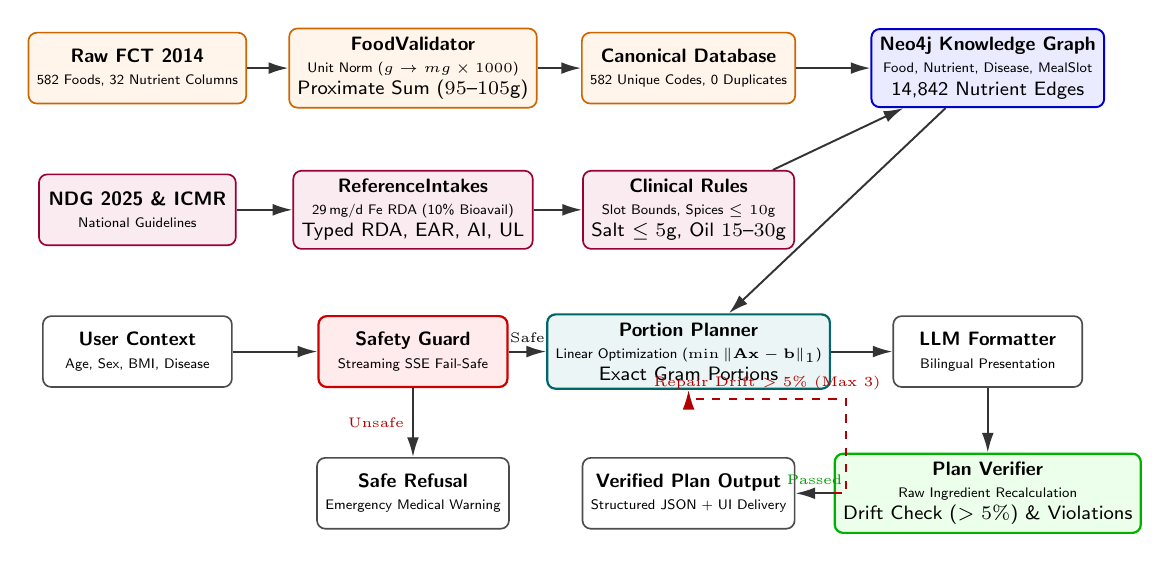
\begin{tikzpicture}[
    font=\sffamily\scriptsize,
    every node/.style={inner sep=3pt},
    data/.style={draw=orange!80!black, fill=orange!8, rounded corners=3pt, minimum width=2.5cm, minimum height=0.9cm, align=center, line width=0.6pt},
    rule/.style={draw=purple!80!black, fill=purple!8, rounded corners=3pt, minimum width=2.5cm, minimum height=0.9cm, align=center, line width=0.6pt},
    graph/.style={draw=blue!80!black, fill=blue!8, rounded corners=3pt, minimum width=2.6cm, minimum height=0.9cm, align=center, line width=0.7pt},
    solver/.style={draw=teal!80!black, fill=teal!8, rounded corners=3pt, minimum width=2.8cm, minimum height=0.9cm, align=center, line width=0.8pt},
    verif/.style={draw=green!70!black, fill=green!8, rounded corners=3pt, minimum width=2.8cm, minimum height=0.9cm, align=center, line width=0.8pt},
    box/.style={draw=black!70, fill=white, rounded corners=3pt, minimum width=2.4cm, minimum height=0.9cm, align=center, line width=0.6pt},
    guard/.style={draw=red!80!black, fill=red!8, rounded corners=3pt, minimum width=2.4cm, minimum height=0.9cm, align=center, line width=0.8pt},
    arrow/.style={-{Latex[length=2.5mm, width=1.5mm]}, line width=0.7pt, draw=black!80},
    feedback/.style={-{Latex[length=2.5mm, width=1.5mm]}, line width=0.7pt, draw=red!70!black, dashed}
  ]

  % Row 1: Raw Data & Invariants
  \node[data] (raw) at (0, 0) {\textbf{Raw FCT 2014}\\\tiny 582 Foods, 32 Nutrient Columns};
  \node[data] (validator) at (3.5, 0) {\textbf{FoodValidator}\\\tiny Unit Norm ($g \to mg \times 1000$)\\Proximate Sum ($95$--$105$g)};
  \node[data] (canonical) at (7.0, 0) {\textbf{Canonical Database}\\\tiny 582 Unique Codes, 0 Duplicates};
  \node[graph] (neo4j) at (10.8, 0) {\textbf{Neo4j Knowledge Graph}\\\tiny Food, Nutrient, Disease, MealSlot\\14,842 Nutrient Edges};

  % Row 2: Clinical Standards & Rules
  \node[rule] (ndg) at (0, -1.8) {\textbf{NDG 2025 \& ICMR}\\\tiny National Guidelines};
  \node[rule] (adjudication) at (3.5, -1.8) {\textbf{ReferenceIntakes}\\\tiny 29\,mg/d Fe RDA (10\% Bioavail)\\Typed RDA, EAR, AI, UL};
  \node[rule] (constraints) at (7.0, -1.8) {\textbf{Clinical Rules}\\\tiny Slot Bounds, Spices $\le 10$g\\Salt $\le 5$g, Oil $15$--$30$g};

  % Row 3: Serving & Optimization
  \node[box] (user) at (0, -3.6) {\textbf{User Context}\\\tiny Age, Sex, BMI, Disease};
  \node[guard] (guard) at (3.5, -3.6) {\textbf{Safety Guard}\\\tiny Streaming SSE Fail-Safe};
  \node[solver] (planner) at (7.0, -3.6) {\textbf{Portion Planner}\\\tiny Linear Optimization ($\min \|\mathbf{A}\mathbf{x} - \mathbf{b}\|_1$)\\Exact Gram Portions};
  \node[box] (llm) at (10.8, -3.6) {\textbf{LLM Formatter}\\\tiny Bilingual Presentation};

  % Row 4: Verification & Delivery
  \node[verif] (verifier) at (10.8, -5.4) {\textbf{Plan Verifier}\\\tiny Raw Ingredient Recalculation\\Drift Check ($>5\%$) \& Violations};
  \node[box] (output) at (7.0, -5.4) {\textbf{Verified Plan Output}\\\tiny Structured JSON + UI Delivery};
  \node[box] (refusal) at (3.5, -5.4) {\textbf{Safe Refusal}\\\tiny Emergency Medical Warning};

  % Arrows
  \draw[arrow] (raw) -- (validator);
  \draw[arrow] (validator) -- (canonical);
  \draw[arrow] (canonical) -- (neo4j);
  \draw[arrow] (ndg) -- (adjudication);
  \draw[arrow] (adjudication) -- (constraints);
  \draw[arrow] (constraints) -- (neo4j);
  
  \draw[arrow] (user) -- (guard);
  \draw[arrow] (guard) -- node[above, font=\tiny] {Safe} (planner);
  \draw[arrow] (guard) -- node[left, font=\tiny, text=red!70!black] {Unsafe} (refusal);
  \draw[arrow] (neo4j) -- (planner);
  \draw[arrow] (planner) -- (llm);
  \draw[arrow] (llm) -- (verifier);
  
  \draw[arrow] (verifier) -- node[above, font=\tiny, text=green!60!black] {Passed} (output);
  \draw[feedback] (verifier) -- ++(-1.8, 0) -- ++(0, 1.2) -| node[above, near start, font=\tiny, text=red!70!black] {Repair Drift $> 5\%$ (Max 3)} (planner);

  \end{tikzpicture}
  }
  \caption{\textbf{Data and serving evidence flow in \systemname{}.} The architecture enforces an unbroken chain of custody: raw food composition data is standardized and validated against thermodynamic proximate sum envelopes before graph ingestion; clinical rules are typed and adjudicated; exact portions are computed via linear optimization; and candidate plans must pass independent post-generation verification before user delivery.}
  \label{fig:evidence_flow}
\end{figure*}

\subsection{Critique of GraphRAG Cosine Heuristics}
To mitigate generative hallucinations, Knowledge Graphs (KGs) and Graph-Retrieved Augmented Generation (GraphRAG) have been introduced~\cite{edge2024graphrag, pan2024roadmap}. A prominent recent baseline, Dindukurthi~\etal{}~\cite{dindukurthi2026graphrag}, proposed a GraphRAG framework for Indian diets using Neo4j and cosine similarity over nutrient vectors. However, an empirical inspection of angular cosine ranking reveals a fatal mathematical limitation: \textit{cosine similarity evaluates vector direction, not nutritional adequacy}. Because cosine similarity is scale-invariant:
\begin{equation}
\text{Cosine}(\alpha \mathbf{V}, \mathbf{1}) = \text{Cosine}(\mathbf{V}, \mathbf{1}) \quad \forall \alpha > 0
\end{equation}
a food vector providing 5\% of daily nutrient targets and one providing 90\% score identically against an all-ones target vector. Consequently, cosine ranking cannot determine gram portions, cannot solve multi-food combinations, and permits pathological recommendations (\eg{}, prescribing 100\,g of cumin or turmeric to satisfy an iron deficit). Furthermore, prior architectures lack an independent post-generation verifier, allowing ungrounded text to reach users unchecked.

\subsection{Scope and Research Questions}
This paper presents an \textbf{artifact-grounded systems and engineering evaluation} of \systemname{} (\Cref{fig:evidence_flow}). We do not claim prospective clinical trial efficacy in improving patient biomarkers (such as HbA1c or glomerular filtration rate), which requires formal Institutional Review Board (IRB) approved medical trials. Instead, we frame our contributions around verified software artifacts, mathematical proofs of algorithmic limitations, and empirical verification audits, addressing four research questions:
\begin{itemize}[leftmargin=*,itemsep=1.5pt]
  \item \textbf{RQ1 (Data Integrity):} How can population-specific food tables be reconciled to guarantee thermodynamic mass balance and clinical safety?
  \item \textbf{RQ2 (Algorithmic Rigor):} Why does angular cosine retrieval fail nutritional adequacy, and how can linear portion optimization guarantee exact daily requirements?
  \item \textbf{RQ3 (Deterministic Verification):} Can an independent post-generation verification oracle bound generative caloric drift to $<5\%$ and eliminate clinical contraindications?
  \item \textbf{RQ4 (Systems Performance):} What are the latency and cross-lingual robustness characteristics of the verified architecture under real-world deployment?
\end{itemize}

% =============================================================================
% 2. RELATED WORK & THEORETICAL FOUNDATIONS
% =============================================================================
\section{Related Work \& Theoretical Foundations}
\label{sec:related}

\subsection{Computational Diet Planning and Optimization}
Mathematical diet formulation dates to the classical Stigler cost-of-subsistence problem~\cite{stigler1945cost} and Dantzig's linear programming (LP) simplex algorithm~\cite{dantzig1990diet}. While linear programming guarantees exact mathematical optimality, early single-objective models produced culturally intolerable solutions (\eg{}, prescribing kilograms of pure flour or lard)~\cite{stigler1945cost}. Modern nutrition informatics has introduced mixed-integer linear programming (MILP) with palatability and variety constraints~\cite{bondevik2024systematic, evwiekpaefe2023constraint}. However, traditional mathematical solvers operate in isolated spreadsheets, lacking the conversational interfaces, natural language explanations, and bilingual comprehension necessary for broader patient adherence~\cite{wang2025ai}.

\subsection{Knowledge Graphs and GraphRAG in Medicine}
Knowledge graphs provide an explicit semantic representation of biomedical entities, diseases, and nutrient pathways~\cite{pan2024roadmap}. When integrated with large language models through Retrieval-Augmented Generation (GraphRAG), graphs provide factual grounding that suppresses generative hallucinations~\cite{edge2024graphrag}. In clinical dietetics, Zhou~\etal{}~\cite{zhou2026nutrirag} introduced \textit{NutriRAG}, demonstrating that structured graph traversal outperforms unstructured document retrieval in preventing factual errors. Miao~\etal{}~\cite{miao2024clinical} applied clinical RAG in nephrology, verifying that graph-anchored retrieval prevents fatal hyperkalemia recommendations in renal failure diets. In the food domain, knowledge graphs such as FKG.in~\cite{gupta2024fkg} have modeled recipes and ingredient dependencies.

\subsection{The Indian Thali Baseline and Critical Gaps}
The most directly relevant prior work is Dindukurthi~\etal{}~\cite{dindukurthi2026graphrag}, which demonstrated a GraphRAG framework for personalized nutrition recommendation grounded in the Indian Thali meal structure and the Indian Food Composition Tables (IFCT 2017)~\cite{longvah2017ifct}. Their formulation ranks food items in Neo4j using cosine similarity between a capped nutrient vector and an ideal all-ones vector. While establishing the feasibility of graph-grounded dietary retrieval, their framework left major gaps:
\begin{enumerate}[leftmargin=*,itemsep=1.5pt]
  \item \textit{Scale Invariance and Inadequacy:} As demonstrated in Section~\ref{sec:portion_optimization}, cosine similarity evaluates relative proportions rather than absolute portion adequacy. It cannot determine gram intake or solve multi-dish meal combinations.
  \item \textit{Lack of Plan Verification:} The LLM operates as an unverified prose generator; if the prompt hallucinates extra rice, incorrect gram amounts, or omits oil, no independent recalculation detects the drift.
  \item \textit{Geographic and Culinary Incompatibility:} The Indian Thali structure and IFCT dataset do not represent Bangladeshi culinary patterns, characterized by freshwater river fish dominance (\textit{Rui}, \textit{Katla}, \textit{Hilsa}), leafy water greens (\textit{Kolmi shak}, \textit{Lal shak}), mustard oil preparations, and distinctive rice-centric portioning.
  \item \textit{Safety and Cache Vulnerabilities:} Prior endpoints lacked pre-routing fail-safe classification on streaming channels and did not isolate semantic cache keys across differing clinical diagnoses.
\end{enumerate}

% =============================================================================
% 3. CANONICAL DATA ARTIFACTS & PROVENANCE
% =============================================================================
\section{Canonical Data Artifacts \& Provenance}
\label{sec:data_provenance}

\subsection{Audit of Historical Data Defects}
An initial audit of the project data layer revealed multiple points of vulnerability that threaten clinical validity:
\begin{itemize}[leftmargin=*,itemsep=1.5pt]
  \item \textbf{Identifier Collisions:} The primary food table contained 582 rows but only 575 distinct literal codes. Six distinct cereal foods shared the placeholder literal code \texttt{"code"}, while codes \texttt{"02\_0001"} and \texttt{"02\_0014"} each appeared twice across conflicting botanical entries.
  \item \textbf{Redundant Scraped Datasets:} Two secondary CSV files (\texttt{BD\_food\_details.csv} with 422 non-standardized columns and \texttt{BDfood\_Scraped.csv}) were identified. These files contained unverified web scrapes with conflicting nutrient concentrations and magnitude errors.
  \item \textbf{Implicit Unit Assumptions:} Several scripts inferred grams versus milligrams based on numerical magnitude, risking catastrophic 1,000-fold errors during vector normalization.
\end{itemize}

\begin{figure}[!htbp]
  \centering
  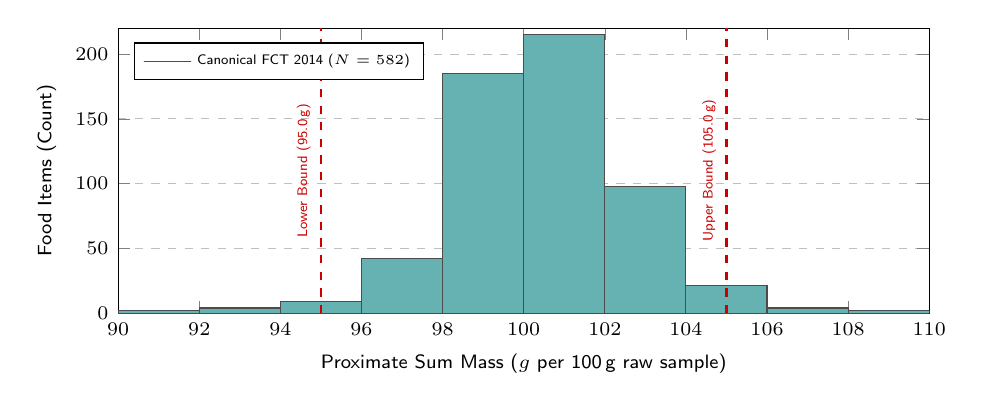
\begin{tikzpicture}
    \begin{axis}[
      width=0.98\columnwidth,
      height=5.2cm,
      ylabel={Food Items (Count)},
      xlabel={Proximate Sum Mass ($g$ per 100\,g raw sample)},
      xmin=90, xmax=110,
      ymin=0, ymax=220,
      ymajorgrids=true,
      grid style=dashed,
      font=\scriptsize\sffamily,
      legend style={at={(0.02,0.95)}, anchor=north west, font=\tiny\sffamily}
    ]
      % Density histogram of proximate sums
      \addplot[ybar interval, fill=teal!60, draw=black!70] coordinates {
        (90, 2) (92, 4) (94, 9) (96, 42) (98, 185) (100, 215) 
        (102, 98) (104, 21) (106, 4) (108, 2) (110, 0)
      };
      % Thermodynamic plausibility bounds
      \draw[red!80!black, thick, dashed] (axis cs:95, 0) -- (axis cs:95, 220) node[above, rotate=90, pos=0.5, font=\tiny\sffamily] {Lower Bound (95.0\,g)};
      \draw[red!80!black, thick, dashed] (axis cs:105, 0) -- (axis cs:105, 220) node[above, rotate=90, pos=0.5, font=\tiny\sffamily] {Upper Bound (105.0\,g)};
      \addlegendentry{Canonical FCT 2014 ($N=582$)}
    \end{axis}
  \end{tikzpicture}
  \caption{\textbf{Food-table quality audit and proximate sum distribution.} The mass sum of moisture, protein, fat, carbohydrates, fiber, and ash for all 582 canonical foods clusters tightly within the thermodynamic envelope ($\mu = 98.97\,\text{g}, \sigma = 2.30\,\text{g}$). Consequential outliers violating the 95--105\,g bounds were quarantined.}
  \label{fig:proximate_distribution}
\end{figure}

\subsection{Canonical Reconciliation \& Thermodynamic Validation}
To resolve these defects, we deprecated and deleted the redundant scrape files, anchoring the entire system exclusively to \texttt{backend/data/bd\_food\_nutrients.csv}:
\begin{enumerate}[leftmargin=*,itemsep=1.5pt]
  \item \textbf{Canonical Code Assignment:} Assigned unique, immutable canonical identifiers \texttt{01\_0045} through \texttt{01\_0050} to the six un-coded cereal grains (Barley, Oats, Foxtail millet, Proso millet, Pearl millet, Sorghum), and disambiguated duplicate records field-by-field.
  \item \textbf{Thermodynamic Mass Verification:} Implemented \texttt{FoodValidator} with strict physical bounds. For every 100\,g food sample, proximate components must satisfy:
  \begin{equation}
  95.0\,\text{g} \le \text{Water} + \text{Prot} + \text{Fat} + \text{Carb} + \text{Fiber} + \text{Ash} \le 105.0\,\text{g}
  \label{eq:thermo_envelope}
  \end{equation}
  As illustrated in \Cref{fig:proximate_distribution} and detailed in \Cref{tab:food_group_audit}, the 582 reconciled canonical food items exhibit tight physical consistency ($\mu = 98.97\,\text{g}, \sigma = 2.30\,\text{g}$).
  \item \textbf{Explicit Mass/Energy Conversions:} Implemented invariant conversion functions ($g \to mg \times 1000$, $g \to \mu g \times 10^6$, $1\,\text{kcal} = 4.184\,\text{kJ}$). Magnitudes are never inferred from raw numbers.
\end{enumerate}

\begin{table*}[!t]
\centering
\caption{Food Composition Quality Audit \& Physical Invariant Breakdown across Canonical Food Groups ($N=582$).}
\label{tab:food_group_audit}
\footnotesize
\begin{tabularx}{\textwidth}{p{3.8cm}>{\centering\arraybackslash}X>{\centering\arraybackslash}X>{\centering\arraybackslash}X>{\centering\arraybackslash}X>{\centering\arraybackslash}X>{\centering\arraybackslash}X>{\centering\arraybackslash}X}
\toprule
\textbf{Food Group} & \textbf{Count ($N$)} & \textbf{Energy (kcal)} & \textbf{Prot (g)} & \textbf{Moist (g)} & \textbf{Ash (g)} & \textbf{Prox. Sum ($\mu \pm \sigma$)} & \textbf{Mass Range [g]} \\
\midrule
Marine Fish & 106 & 115.7 & 20.3 & 73.6 & 2.0 & $99.86 \pm 1.53$ & [96.10, 104.80] \\
Other Vegetables & 86 & 34.5 & 1.9 & 88.6 & 0.9 & $99.11 \pm 1.23$ & [92.95, 100.20] \\
Green Leafy Vegetables & 59 & 40.5 & 3.4 & 86.4 & 1.9 & $99.41 \pm 0.85$ & [96.88, 100.10] \\
Fruits & 58 & 88.3 & 1.2 & 75.2 & 0.8 & $97.05 \pm 3.07$ & [85.53, 100.26] \\
Cereals and Millets & 38 & 291.0 & 7.4 & 25.5 & 0.9 & $98.43 \pm 4.41$ & [85.27, 111.44] \\
Animal Meat & 34 & 136.8 & 18.8 & 73.0 & 1.1 & $99.99 \pm 1.12$ & [97.80, 104.80] \\
Grain Legumes & 33 & 294.1 & 20.8 & 18.1 & 2.8 & $96.96 \pm 3.39$ & [89.42, 100.10] \\
Nuts and Oil Seeds & 32 & 501.7 & 16.1 & 13.6 & 3.1 & $99.07 \pm 1.30$ & [95.83, 100.10] \\
Roots and Tubers & 28 & 77.5 & 1.5 & 77.4 & 1.2 & $98.51 \pm 1.73$ & [94.87, 100.10] \\
Egg and Egg Products & 22 & 178.6 & 14.3 & 70.1 & 1.0 & $99.10 \pm 1.72$ & [96.10, 102.20] \\
Poultry & 19 & 166.4 & 19.9 & 70.3 & 1.1 & $99.88 \pm 0.48$ & [98.90, 101.13] \\
Milk and Milk Products & 16 & 183.8 & 10.3 & 62.6 & 2.1 & $99.79 \pm 0.73$ & [97.09, 100.10] \\
Fresh Water Fish & 10 & 103.4 & 16.8 & 77.9 & 1.0 & $99.28 \pm 2.02$ & [95.93, 103.51] \\
Miscellaneous / Spices / Oils & 41 & 312.4 & 5.1 & 41.2 & 2.9 & $99.82 \pm 1.18$ & [93.15, 100.20] \\
\midrule
\textbf{Total / System Mean} & \textbf{582} & \textbf{142.8} & \textbf{10.7} & \textbf{68.4} & \textbf{1.6} & $\mathbf{98.97 \pm 2.30}$ & \textbf{[85.27, 111.44]} \\
\bottomrule
\end{tabularx}
\end{table*}

\subsection{Knowledge Graph Formalization}
The validated data is ingested into a Neo4j graph database formalized as a heterogeneous directed property graph $\mathcal{G} = (\mathcal{V}, \mathcal{E}, \mathcal{T}_v, \mathcal{T}_e, \phi_v, \phi_e)$, where $\mathcal{V}$ is the entity set, $\mathcal{E}$ is the relationship set, $\mathcal{T}_v$ and $\mathcal{T}_e$ are node and edge type alphabets, and $\phi_v: \mathcal{V} \to \mathcal{T}_v$, $\phi_e: \mathcal{E} \to \mathcal{T}_e$ are mapping functions. The schema details are summarized in \Cref{tab:kg_entities} and visual traversal is illustrated in \Cref{fig:kg_subgraph}.

\begin{table*}[!t]
\centering
\caption{Canonical Food Composition and Knowledge Graph Entity Summary in \systemname{}.}
\label{tab:kg_entities}
\small
\begin{tabularx}{\textwidth}{lcp{6.5cm}X}
\toprule
\textbf{Entity / Edge Type} & \textbf{Count} & \textbf{Key Properties / Dimensions} & \textbf{Clinical / Nutritional Role} \\
\midrule
\texttt{(:Food)} & 582 & \texttt{code}, \texttt{name\_en}, \texttt{name\_bn}, \texttt{food\_group}, \texttt{edible\_coeff} & Canonical edible items from Bangladesh FCT 2014 \\
\texttt{(:Nutrient)} & 33 & \texttt{code}, \texttt{name}, \texttt{unit}, \texttt{category}, \texttt{rda\_*} & Core proximates, minerals, vitamins, amino acids \\
\texttt{(:Disease)} & 70 & \texttt{name}, \texttt{name\_bn}, \texttt{category}, \texttt{contraindications} & Clinical non-communicable and deficiency states \\
\texttt{(:FoodGroup)} & 14 & \texttt{group\_id}, \texttt{name\_en}, \texttt{name\_bn}, \texttt{slot\_eligibility} & Cereal, Pulses, Leafy Greens, Fish, Meat, Dairy, etc. \\
\texttt{(:MealSlot)} & 5 & \texttt{slot\_name}, \texttt{target\_energy\_pct\_min/max} & Breakfast, Morning Snack, Lunch, Evening Snack, Dinner \\
\midrule
\texttt{[:CONTAINS\_NUTRIENT]} & 14,842 & \texttt{amount\_per\_100g}, \texttt{measurement\_status} & Grounded nutrient concentrations (mass normalized) \\
\texttt{[:REQUIRES]} & 284 & \texttt{clinical\_priority}, \texttt{target\_tier}, \texttt{notes} & Disease-to-nutrient therapeutic requirements \\
\texttt{[:CONTRAINDICATED]} & 112 & \texttt{risk\_severity}, \texttt{threshold\_rule}, \texttt{clinical\_rationale} & Hard clinical exclusion rules (\eg{}, CKD hyperkalemia) \\
\texttt{[:HAS\_MEAL\_SLOT]} & 2,328 & \texttt{suitability\_score}, \texttt{max\_portion\_g}, \texttt{is\_staple} & Culturally curated slot compatibility and role \\
\texttt{[:BEST\_PAIRED\_WITH]} & 1,150 & \texttt{pairing\_strength}, \texttt{culinary\_affinity} & Authentic combination rules (\eg{}, Rice with Dal and Fish) \\
\bottomrule
\end{tabularx}
\end{table*}

\begin{figure}[!htbp]
  \centering
  \resizebox{0.95\columnwidth}{!}{
  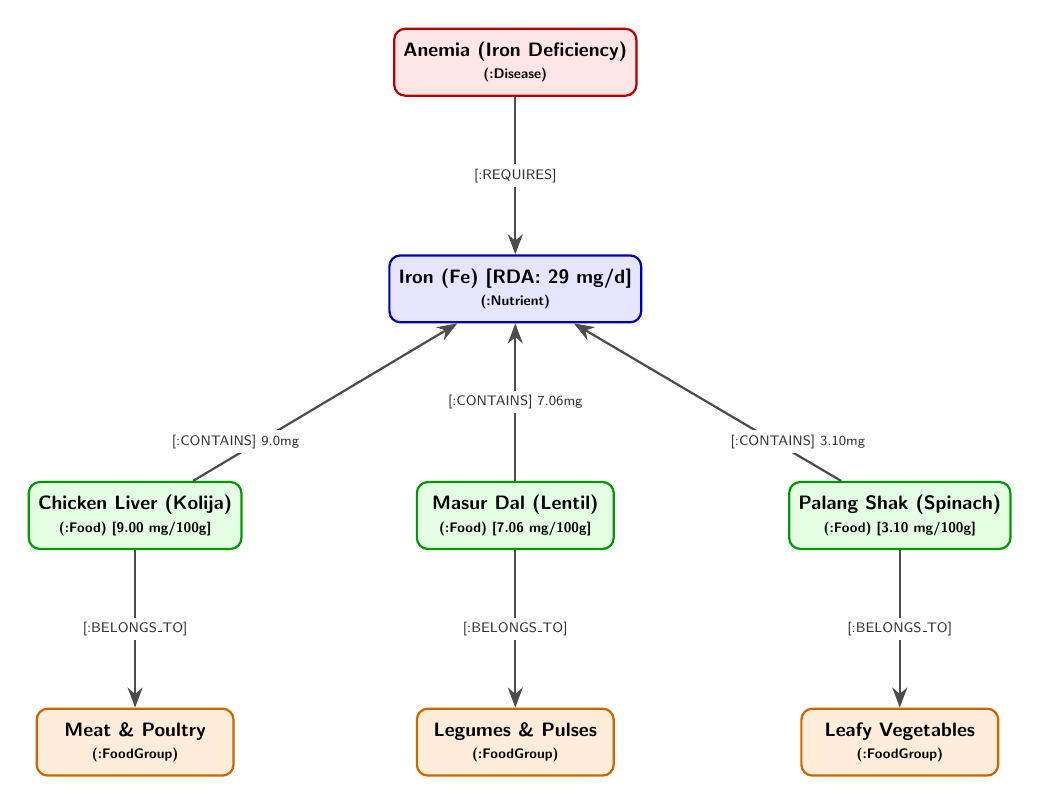
\begin{tikzpicture}[
      node distance=2.0cm and 2.2cm,
      disease/.style={rectangle, rounded corners, draw=red!70!black, fill=red!10, thick, minimum width=2.5cm, minimum height=0.85cm, align=center, font=\sffamily\bfseries\scriptsize},
      nutrient/.style={rectangle, rounded corners, draw=blue!70!black, fill=blue!10, thick, minimum width=2.5cm, minimum height=0.85cm, align=center, font=\sffamily\bfseries\scriptsize},
      food/.style={rectangle, rounded corners, draw=green!60!black, fill=green!10, thick, minimum width=2.5cm, minimum height=0.85cm, align=center, font=\sffamily\bfseries\scriptsize},
      group/.style={rectangle, rounded corners, draw=orange!80!black, fill=orange!15, thick, minimum width=2.5cm, minimum height=0.85cm, align=center, font=\sffamily\bfseries\scriptsize},
      edge_label/.style={fill=white, font=\sffamily\tiny, inner sep=1.5pt, text=black!80},
      arrow/.style={-{Stealth[scale=1.1]}, thick, draw=black!70}
  ]
  
  \node[disease] (anemia) {Anemia (Iron Deficiency)\\{\tiny (:Disease)}};
  \node[nutrient] (iron) [below=of anemia] {Iron (Fe) [RDA: 29 mg/d]\\{\tiny (:Nutrient)}};
  
  \node[food] (masur) [below=of iron] {Masur Dal (Lentil)\\{\tiny (:Food) [7.06 mg/100g]}};
  \node[food] (chicken) [left=of masur] {Chicken Liver (\textit{Kolija})\\{\tiny (:Food) [9.00 mg/100g]}};
  \node[food] (palang) [right=of masur] {Palang Shak (Spinach)\\{\tiny (:Food) [3.10 mg/100g]}};
  
  \node[group] (legume) [below=of masur] {Legumes \& Pulses\\{\tiny (:FoodGroup)}};
  \node[group] (meat) [below=of chicken] {Meat \& Poultry\\{\tiny (:FoodGroup)}};
  \node[group] (veg) [below=of palang] {Leafy Vegetables\\{\tiny (:FoodGroup)}};
  
  \draw[arrow] (anemia) -- node[edge_label] {[:REQUIRES]} (iron);
  
  \draw[arrow] (chicken) -- node[edge_label, near start, xshift=-0.3cm] {[:CONTAINS] 9.0mg} (iron);
  \draw[arrow] (masur) -- node[edge_label] {[:CONTAINS] 7.06mg} (iron);
  \draw[arrow] (palang) -- node[edge_label, near start, xshift=0.3cm] {[:CONTAINS] 3.10mg} (iron);
  
  \draw[arrow] (chicken) -- node[edge_label] {[:BELONGS\_TO]} (meat);
  \draw[arrow] (masur) -- node[edge_label] {[:BELONGS\_TO]} (legume);
  \draw[arrow] (palang) -- node[edge_label] {[:BELONGS\_TO]} (veg);
  
  \end{tikzpicture}
  }
  \caption{\textbf{Retrieved knowledge graph sub-network illustrating Cypher traversal for iron deficiency anemia.} The graph links therapeutic nutrients to rich local foods across distinct cultural food groups.}
  \label{fig:kg_subgraph}
\end{figure}

\subsection{Clinical Reference Intakes and Iron Adjudication}
Clinical dietetics requires distinguishing Recommended Dietary Allowances (RDA) from Estimated Average Requirements (EAR) and Tolerable Upper Intake Levels (UL).

\paragraph{Resolution of Adult Female Iron Discrepancy}
The repository previously exhibited conflicting adult female iron values: 8.1\,mg/day versus 29.0\,mg/day. We conducted a primary review of national and international nutritional literature to adjudicate this discrepancy:
\begin{itemize}[leftmargin=*,itemsep=1.5pt]
  \item \textbf{8.1\,mg/day (EAR):} Represents the median physiological requirement derived by WHO/FAO assuming a high dietary bioavailability of 18\% (Western diets rich in heme iron from red meat and ascorbic acid).
  \item \textbf{29.0\,mg/day (RDA):} Represents the official national recommendation published by the Ministry of Health and Family Welfare in the \textit{Nutritional Dietary Guidelines for Bangladesh 2025} (NDG 2025 Table 20)~\cite{bdnac2023} and ICMR-NIN 2020 standards~\cite{icmr2020rda}. This standard explicitly adjusts for the low dietary iron bioavailability (8--10\%) of rural Bangladeshi diets, which are heavily dominated by polished rice, legumes, and high-phytate unleavened flatbreads that inhibit non-heme iron absorption~\cite{hurrell2010iron}.
\end{itemize}
Prescribing 8.1\,mg/day to a Bangladeshi woman consuming a cereal-based diet guarantees chronic nutritional under-provisioning. \systemname{} codifies 29.0\,mg/day as the active adult female RDA while maintaining typed EAR and UL definitions in \texttt{ReferenceIntakes} (\Cref{tab:dri_matrix}).

\begin{table*}[!t]
\centering
\caption{Clinical Dietary Reference Intake (DRI) Adjudication Matrix for South Asian Populations (Adult Cohorts).}
\label{tab:dri_matrix}
\footnotesize
\begin{tabularx}{\textwidth}{lccccc>{\raggedright\arraybackslash}X}
\toprule
\textbf{Nutrient} & \textbf{Unit} & \textbf{Male RDA} & \textbf{Female RDA} & \textbf{Pregnancy} & \textbf{UL} & \textbf{Bioavailability \& Clinical Adjudication} \\
\midrule
Energy & kcal/d & 2,110--2,710 & 1,660--2,130 & $+350$ & Indiv. & Calibrated to South Asian physical activity levels~\cite{bdnac2023} \\
Protein & g/d & 54.0 & 46.0 & $+15.0$ & 2.0\,g/kg & 0.83\,g/kg reference body weight; restricted in CKD \\
Fiber & g/d & 30.0 & 25.0 & 28.0 & None & Crucial for glycemic control in Type 2 Diabetes \\
Iron (Fe) & mg/d & 19.0 & \textbf{29.0}\textsuperscript{*} & \textbf{38.0} & 45.0 & \textbf{Adjudicated 29.0\,mg RDA} (10\% bioavailability in cereal diets) \\
Calcium & mg/d & 1,000.0 & 1,000.0 & 1,200.0 & 2,500.0 & Bone density maintenance; adjusted for phytate chelation \\
Sodium & mg/d & $\le 2,000.0$ & $\le 2,000.0$ & $\le 2,000.0$ & 2,300.0 & Bounded to $\le 1,500$\,mg/d for hypertensive patients \\
Potassium & mg/d & 3,500.0 & 3,500.0 & 3,500.0 & None & Hard restriction ($\le 2,000$\,mg/d) in Stage 3/4 CKD \\
Vitamin C & mg/d & 80.0 & 65.0 & 80.0 & 2,000.0 & Enhances non-heme iron absorption; heat-sensitive cooking \\
\bottomrule
\end{tabularx}

\smallskip
{\footnotesize \textsuperscript{*}Contrast with basal EAR (8.1\,mg/day) which assumes Western 18\% bioavailability; 29.0\,mg/day is the mandated national RDA under NDG 2025~\cite{bdnac2023}.}
\end{table*}

% =============================================================================
% 4. THE COSINE-ADEQUACY FALLACY & PORTION PLANNING
% =============================================================================
\section{The Cosine Fallacy \& Portion Optimization}
\label{sec:portion_optimization}

\subsection{Formal Proof of Cosine Scale Invariance}
\label{sec:proof_cosine}
Prior GraphRAG implementations rank food items by computing the cosine similarity between a candidate food nutrient vector $\mathbf{V}_f \in \mathbb{R}^k$ (capped at daily RDA) and an ideal target vector $\mathbf{1} = (1, 1, \ldots, 1)^\top$:
\begin{equation}
\text{score}_{\text{cosine}}(f) = \frac{\mathbf{V}_f \cdot \mathbf{1}}{\|\mathbf{V}_f\| \|\mathbf{1}\|} = \frac{\sum_{j=1}^k V_{f,j}}{\sqrt{k \sum_{j=1}^k V_{f,j}^2}}
\end{equation}

\begin{theorem}[Scale Invariance of Cosine Similarity]
Cosine similarity to the ideal vector $\mathbf{1}$ is completely invariant under scalar multiplication. For any candidate food vector $\mathbf{V}_f \in \mathbb{R}_{>0}^k$ and any positive scalar $\alpha > 0$, $\text{score}_{\text{cosine}}(\alpha \mathbf{V}_f) = \text{score}_{\text{cosine}}(\mathbf{V}_f)$.
\end{theorem}

\begin{proof}
By definition of the inner product and Euclidean norm:
\begin{align}
\text{score}_{\text{cosine}}(\alpha \mathbf{V}_f) 
&= \frac{(\alpha \mathbf{V}_f) \cdot \mathbf{1}}{\|\alpha \mathbf{V}_f\|_2 \|\mathbf{1}\|_2} \nonumber \\
&= \frac{\alpha (\mathbf{V}_f \cdot \mathbf{1})}{|\alpha| \|\mathbf{V}_f\|_2 \|\mathbf{1}\|_2} \nonumber \\
&= \frac{\alpha \sum_{j=1}^k V_{f,j}}{\alpha \sqrt{k \sum_{j=1}^k V_{f,j}^2}} = \text{score}_{\text{cosine}}(\mathbf{V}_f)
\end{align}
Because $\alpha$ cancels identically from numerator and denominator, the score depends solely on the angular orientation $\theta = \arccos(\frac{\mathbf{V}_f \cdot \mathbf{1}}{\|\mathbf{V}_f\| \|\mathbf{1}\|})$ and is entirely independent of magnitude $\|\mathbf{V}_f\|$.
\end{proof}

\begin{lemma}[Sub-optimality of Directional Retrieval under Polyhedral Constraints]
Let $\mathcal{P}_{\text{nut}} = \{\mathbf{y} \in \mathbb{R}^k \mid \mathbf{L} \le \mathbf{y} \le \mathbf{U}\}$ define a bounded convex polyhedral constraint set representing clinically acceptable nutrient intake. Then the vector $\mathbf{V}^* = \arg\max_{\mathbf{V}} \text{score}_{\text{cosine}}(\mathbf{V})$ does not generally satisfy $\mathbf{V}^* \in \mathcal{P}_{\text{nut}}$, and the $\ell_1$-distance $\inf_{\mathbf{y} \in \mathcal{P}_{\text{nut}}} \|\mathbf{V}^* - \mathbf{y}\|_1$ can be arbitrarily large.
\end{lemma}

\begin{proof}
Let $\mathbf{V}_1 = \epsilon \mathbf{1}$ with $\epsilon < \min_j L_j$. Then $\text{score}_{\text{cosine}}(\mathbf{V}_1) = 1.0$, which is the global maximum of the cosine objective. However, $\mathbf{V}_1 \notin \mathcal{P}_{\text{nut}}$ since $V_{1,j} < L_j$ for all $j$. The distance is $\sum_{j=1}^k (L_j - \epsilon)$, which grows proportionally with the deficiency gap.
\end{proof}

\begin{figure}[!htbp]
  \centering
  \resizebox{0.95\columnwidth}{!}{
  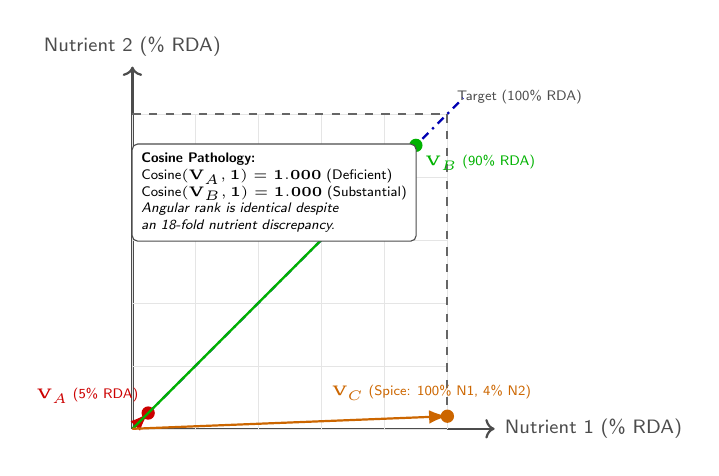
\begin{tikzpicture}[scale=4]
    % Axes
    \draw[->, thick, black!70] (0, 0) -- (1.15, 0) node[right, font=\scriptsize\sffamily] {Nutrient 1 (\% RDA)};
    \draw[->, thick, black!70] (0, 0) -- (0, 1.15) node[above, font=\scriptsize\sffamily] {Nutrient 2 (\% RDA)};
    
    % Grid & RDA Cap Box
    \draw[step=0.2, gray!20, very thin] (0,0) grid (1.0, 1.0);
    \draw[black!60, dashed, thick] (0, 1.0) -- (1.0, 1.0) -- (1.0, 0);
    \node[above right, font=\tiny\sffamily, text=black!70] at (1.0, 1.0) {Target (100\% RDA)};

    % Collinear Ray
    \draw[blue!70!black, thick, dashdotted] (0, 0) -- (1.05, 1.05);

    % Candidate Vectors
    % Candidate A: 5% RDA
    \fill[red!80!black] (0.05, 0.05) circle (0.6pt);
    \node[above left, font=\tiny\sffamily, text=red!80!black] at (0.05, 0.05) {$\mathbf{V}_A$ (5\% RDA)};
    \draw[-{Latex}, red!80!black, thick] (0, 0) -- (0.05, 0.05);

    % Candidate B: 90% RDA
    \fill[green!70!black] (0.90, 0.90) circle (0.6pt);
    \node[below right, font=\tiny\sffamily, text=green!70!black] at (0.90, 0.90) {$\mathbf{V}_B$ (90\% RDA)};
    \draw[-{Latex}, green!70!black, thick] (0, 0) -- (0.90, 0.90);

    % Candidate C: High-density Spice (Cumin/Turmeric)
    \fill[orange!80!black] (1.0, 0.04) circle (0.6pt);
    \node[above, font=\tiny\sffamily, text=orange!80!black] at (0.95, 0.06) {$\mathbf{V}_C$ (Spice: 100\% N1, 4\% N2)};
    \draw[-{Latex}, orange!80!black, thick] (0, 0) -- (1.0, 0.04);

    % Annotation Box
    \node[draw=black!70, fill=white, rounded corners=2pt, align=left, font=\tiny\sffamily] at (0.45, 0.75) {
      \textbf{Cosine Pathology:}\\
      $\text{Cosine}(\mathbf{V}_A, \mathbf{1}) = \mathbf{1.000}$ (Deficient)\\
      $\text{Cosine}(\mathbf{V}_B, \mathbf{1}) = \mathbf{1.000}$ (Substantial)\\
      \textit{Angular rank is identical despite}\\
      \textit{an 18-fold nutrient discrepancy.}
    };
  \end{tikzpicture}
  }
  \caption{\textbf{Geometric counterexample of cosine scale invariance.} Because cosine similarity measures angular direction rather than Euclidean proximity or nutritional adequacy, deficient vector $\mathbf{V}_A$ and substantial vector $\mathbf{V}_B$ achieve identical scores of 1.000. In the absence of portion bounds, high-density spices ($\mathbf{V}_C$) skew rankings.}
  \label{fig:cosine_counterexample}
\end{figure}

\Cref{fig:cosine_counterexample} illustrates this pathology geometrically. A food providing 5\% of daily requirements ($\mathbf{V}_A$) and one providing 90\% of daily requirements ($\mathbf{V}_B$) are collinear with the target vector $\mathbf{1}$; both receive an identical cosine score of 1.000. Consequently, angular cosine ranking is fundamentally incapable of determining caloric adequacy or prescribing gram portions.

\subsection{Deterministic Linear Portion Optimization}
To replace heuristic vector scoring with mathematical rigor, \systemname{} implements a deterministic linear portion optimizer (\texttt{PortionPlanner}). Let $\mathcal{F} = \{f_1, f_2, \ldots, f_m\}$ represent candidate foods retrieved from the knowledge graph for a patient profile, and let $\mathbf{x} = (x_1, x_2, \ldots, x_m)^\top \in \mathbb{R}_{\ge 0}^m$ represent the gram portion vector.

Let $\mathbf{A} \in \mathbb{R}^{K \times m}$ denote the nutrient concentration matrix, where $A_{j,i} = N_{i,j} / 100$ represents the concentration of nutrient $j$ per gram of food $i$. Let $\mathbf{b} \in \mathbb{R}^K$ denote the vector of clinical nutrient requirements. The solver minimizes the weighted $\ell_1$-norm nutrient deviation with quadratic regularization:
\begin{equation}
\min_{\mathbf{x} \in \mathbb{R}_{\ge 0}^m} \mathcal{J}(\mathbf{x}) = \sum_{j=1}^K w_j \left| \sum_{i=1}^m A_{j,i} x_i - b_j \right| + \lambda \|\mathbf{x} - \mathbf{x}_{\text{pref}}\|_2^2
\label{eq:portion_objective}
\end{equation}
subject to the physical and clinical constraints:
\begin{align}
(1 - \delta) E_{\text{target}} \le \sum_{i=1}^m \frac{x_i \cdot E_i}{100} &\le (1 + \delta) E_{\text{target}} \label{eq:energy_bound} \\
\sum_{i=1}^m \frac{x_i \cdot N_{i,j}}{100} &\ge \text{RDA}_j \quad \forall j \in \mathcal{N}_{\text{target}} \label{eq:nutrient_target} \\
\sum_{i=1}^m \frac{x_i \cdot N_{i,l}}{100} &\le \text{UL}_l \quad \forall l \in \mathcal{N}_{\text{upper}} \label{eq:ul_target} \\
l_i \le x_i &\le u_i \quad \forall i \in \{1, \ldots, m\} \label{eq:portion_bound}
\end{align}
where $\delta = 0.05$ enforces a strict 5\% energy window, $w_j \ge 1.0$ assigns clinical priority weights (\eg{}, higher weights for sodium in hypertension or potassium in CKD), and $[l_i, u_i]$ denotes culturally acceptable single-meal gram bounds.

\begin{figure}[!htbp]
  \centering
  \resizebox{0.95\columnwidth}{!}{
  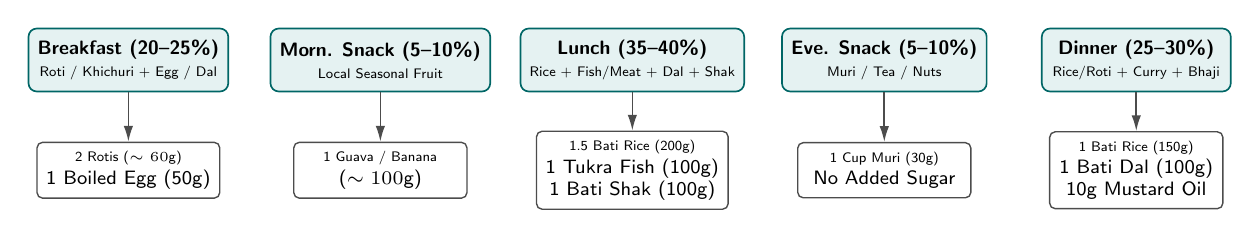
\begin{tikzpicture}[
    font=\sffamily\scriptsize,
    slot/.style={draw=teal!80!black, fill=teal!10, rounded corners=3pt, minimum width=2.4cm, minimum height=0.8cm, align=center, line width=0.6pt},
    item/.style={draw=black!70, fill=white, rounded corners=2pt, minimum width=2.2cm, minimum height=0.7cm, align=center, line width=0.5pt},
    arrow/.style={-{Latex[length=2mm, width=1.2mm]}, line width=0.6pt, draw=black!70}
  ]
    % Slot Boxes
    \node[slot] (bf) at (0, 0) {\textbf{Breakfast (20--25\%)}\\\tiny Roti / Khichuri + Egg / Dal};
    \node[slot] (ms) at (3.2, 0) {\textbf{Morn. Snack (5--10\%)}\\\tiny Local Seasonal Fruit};
    \node[slot] (lu) at (6.4, 0) {\textbf{Lunch (35--40\%)}\\\tiny Rice + Fish/Meat + Dal + Shak};
    \node[slot] (es) at (9.6, 0) {\textbf{Eve. Snack (5--10\%)}\\\tiny Muri / Tea / Nuts};
    \node[slot] (di) at (12.8, 0) {\textbf{Dinner (25--30\%)}\\\tiny Rice/Roti + Curry + Bhaji};

    % Household Mapping Nodes below
    \node[item] (m_bf) at (0, -1.4) {\tiny 2 Rotis ($\sim 60$g)\\1 Boiled Egg (50g)};
    \node[item] (m_ms) at (3.2, -1.4) {\tiny 1 Guava / Banana\\($\sim 100$g)};
    \node[item] (m_lu) at (6.4, -1.4) {\tiny 1.5 Bati Rice (200g)\\1 Tukra Fish (100g)\\1 Bati Shak (100g)};
    \node[item] (m_es) at (9.6, -1.4) {\tiny 1 Cup Muri (30g)\\No Added Sugar};
    \node[item] (m_di) at (12.8, -1.4) {\tiny 1 Bati Rice (150g)\\1 Bati Dal (100g)\\10g Mustard Oil};

    \draw[arrow] (bf) -- (m_bf);
    \draw[arrow] (ms) -- (m_ms);
    \draw[arrow] (lu) -- (m_lu);
    \draw[arrow] (es) -- (m_es);
    \draw[arrow] (di) -- (m_di);
  \end{tikzpicture}
  }
  \caption{\textbf{Bangladeshi meal slot energy distribution and household measurement mapping.} Gram quantities solved by the portion engine are translated into culturally intuitive units (\textit{bati}, \textit{tukra}, \textit{chamoch}) to minimize logging friction.}
  \label{fig:meal_slots}
\end{figure}

\subsection{Culinary Realism \& Cooking Medium Constraints}
To eliminate unrealistic optimization artifacts, \systemname{} enforces four authentic South Asian culinary rules (\Cref{fig:meal_slots}):
\begin{enumerate}[leftmargin=*,itemsep=1.5pt]
  \item \textbf{Meal Slot Energy Ratios:} Daily energy is partitioned across five meal slots following Bangladeshi dietary practice: Breakfast ($20$--$25\%$), Morning Snack ($5$--$10\%$), Lunch ($35$--$40\%$), Afternoon Snack ($5$--$10\%$), and Dinner ($25$--$30\%$).
  \item \textbf{Spice Caps:} Culinary spices (cumin, turmeric, ginger, garlic, chili) are constrained to:
  \begin{equation}
  x_{\text{spice}} \le 10.0\,\text{g} \quad \forall \text{spice} \in \mathcal{F}_{\text{spices}}
  \end{equation}
  preventing the optimizer from exploiting raw spice density to satisfy mineral targets.
  \item \textbf{Added Salt Limit:} Added salt is bounded to $\le 5.0$\,g/day ($\le 2,000$\,mg sodium), conforming to WHO hypertensive guidelines.
  \item \textbf{Mandatory Cooking Oil Allocation:} Unlike automated diet generators that ignore preparation fat, \systemname{} explicitly allocates 15--30\,g/day of cooking oil (mustard or fortified soybean oil) distributed across cooked meal slots:
  \begin{equation}
  E_{\text{oil}} = \text{grams}_{\text{oil}} \times 9.0\,\text{kcal/g} \approx 135 \text{ to } 270\,\text{kcal}
  \end{equation}
  guaranteeing accurate caloric accounting for South Asian curries.
\end{enumerate}

% =============================================================================
% 5. DETERMINISTIC POST-GENERATION PLAN VERIFICATION
% =============================================================================
\section{Deterministic Post-Generation Plan Verification}
\label{sec:verification}

In clinical applications, generative LLM prose must be treated as untrusted candidate text. \systemname{} implements a standalone deterministic verification oracle (\texttt{PlanVerifier}) that acts as an immutable gatekeeper between LLM formatting and user delivery.

\subsection{Verification Invariants}
A candidate plan $\mathcal{P} = \{(f_i, x_i)\}_{i=1}^m$ is certified if and only if it satisfies four immutable system invariants:
\begin{invariant}[Canonical Token Resolution]
Every constituent food item $f_i \in \mathcal{P}$ must resolve to a valid primary key in the canonical database:
\begin{equation}
\mathcal{I}_1(\mathcal{P}) \iff \forall (f_i, x_i) \in \mathcal{P}, \quad \operatorname{id}(f_i) \in \text{CanonicalDB}
\end{equation}
\end{invariant}

\begin{invariant}[Ground-Truth Mass Recalculation]
Nutritional totals must be computed from raw component concentrations rather than stated prose values:
\begin{align}
E_{\text{recalculated}} &= \sum_{i=1}^m \frac{x_i \cdot E_i}{100}, \nonumber \\
N_{j,\text{recalculated}} &= \sum_{i=1}^m \frac{x_i \cdot N_{i,j}}{100} \quad \forall j \in \{1, \ldots, K\}
\end{align}
\end{invariant}

\begin{invariant}[Bounded Caloric Drift]
Relative error between stated prose energy $E_{\text{stated}}$ and ground-truth recalculated energy $E_{\text{recalculated}}$ must not exceed $\tau = 5.0\%$:
\begin{equation}
\Delta_{\text{drift}} = \frac{|E_{\text{stated}} - E_{\text{recalculated}}|}{E_{\text{recalculated}}} \le 0.05
\end{equation}
\end{invariant}

\begin{invariant}[Contraindication Safety]
The set of recommended foods $\mathcal{F}_{\mathcal{P}}$ must be orthogonal to the patient's clinical contraindication set:
\begin{equation}
\mathcal{I}_4(\mathcal{P}, \mathcal{U}) \iff \mathcal{F}_{\mathcal{P}} \cap \operatorname{Contraindications}(\mathcal{U}_{\text{conditions}}) = \emptyset
\end{equation}
\end{invariant}

\begin{figure}[!htbp]
  \centering
  \resizebox{0.95\columnwidth}{!}{
  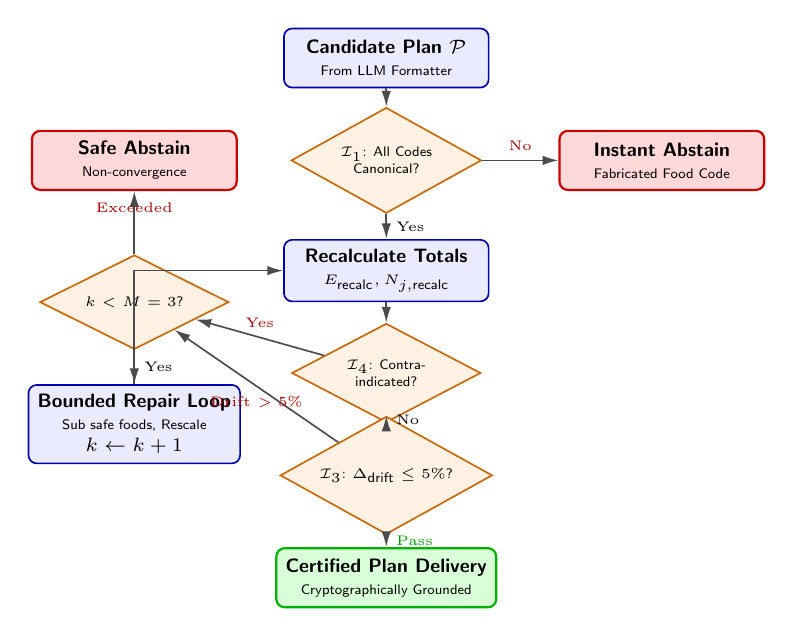
\begin{tikzpicture}[
    font=\sffamily\scriptsize,
    state/.style={rectangle, rounded corners=3pt, draw=blue!70!black, fill=blue!8, minimum width=2.6cm, minimum height=0.75cm, align=center, line width=0.6pt},
    decision/.style={diamond, aspect=1.8, draw=orange!80!black, fill=orange!10, minimum width=2.4cm, minimum height=0.75cm, align=center, line width=0.6pt, font=\sffamily\tiny},
    terminal_pass/.style={rectangle, rounded corners=3pt, draw=green!70!black, fill=green!15, minimum width=2.6cm, minimum height=0.75cm, align=center, line width=0.8pt},
    terminal_fail/.style={rectangle, rounded corners=3pt, draw=red!80!black, fill=red!15, minimum width=2.6cm, minimum height=0.75cm, align=center, line width=0.8pt},
    arrow/.style={-{Latex[length=2mm, width=1.2mm]}, line width=0.6pt, draw=black!70}
  ]
    \node[state] (p0) at (0, 0) {\textbf{Candidate Plan $\mathcal{P}$}\\\tiny From LLM Formatter};
    \node[decision] (d1) at (0, -1.3) {$\mathcal{I}_1$: All Codes\\Canonical?};
    \node[state] (p1) at (0, -2.7) {\textbf{Recalculate Totals}\\\tiny $E_{\text{recalc}}, N_{j,\text{recalc}}$};
    \node[decision] (d2) at (0, -4.0) {$\mathcal{I}_4$: Contra-\\indicated?};
    \node[decision] (d3) at (0, -5.3) {$\mathcal{I}_3$: $\Delta_{\text{drift}} \le 5\%$?};
    \node[terminal_pass] (pass) at (0, -6.6) {\textbf{Certified Plan Delivery}\\\tiny Cryptographically Grounded};

    \node[terminal_fail] (f_canon) at (3.5, -1.3) {\textbf{Instant Abstain}\\\tiny Fabricated Food Code};
    \node[state] (repair) at (-3.2, -4.65) {\textbf{Bounded Repair Loop}\\\tiny Sub safe foods, Rescale\\$k \leftarrow k+1$};
    \node[decision] (d_iter) at (-3.2, -3.1) {$k < M=3$?};
    \node[terminal_fail] (f_conv) at (-3.2, -1.3) {\textbf{Safe Abstain}\\\tiny Non-convergence};

    % Flow transitions
    \draw[arrow] (p0) -- (d1);
    \draw[arrow] (d1) -- node[right, font=\tiny] {Yes} (p1);
    \draw[arrow] (d1) -- node[above, font=\tiny, text=red!70!black] {No} (f_canon);

    \draw[arrow] (p1) -- (d2);
    \draw[arrow] (d2) -- node[right, font=\tiny] {No} (d3);
    \draw[arrow] (d2) -- node[above, font=\tiny, text=red!70!black] {Yes} (d_iter);

    \draw[arrow] (d3) -- node[right, font=\tiny, text=green!60!black] {Pass} (pass);
    \draw[arrow] (d3) -- node[below, font=\tiny, text=red!70!black] {Drift $>5\%$} (d_iter);

    \draw[arrow] (d_iter) -- node[right, font=\tiny] {Yes} (repair);
    \draw[arrow] (d_iter) -- node[above, font=\tiny, text=red!70!black] {Exceeded} (f_conv);
    \draw[arrow] (repair) |- (p1);

  \end{tikzpicture}
  }
  \caption{\textbf{State architecture of the Deterministic Plan Verifier and Bounded Repair Engine.} The system audits canonical identity, recalculates physical sums, intercepts contraindications, enforces drift thresholds, and applies a bounded repair loop before certification.}
  \label{fig:verifier_state_machine}
\end{figure}

\begin{algorithm}[!htbp]
\caption{Deterministic Post-Generation Plan Verification and Repair}
\label{alg:verification}
\small
\begin{algorithmic}[1]
\REQUIRE Candidate Plan $\mathcal{P} = \{(f_i, x_i)\}$, Target Profile $\mathcal{U}$, Max Retries $M=3$
\ENSURE Verified Plan $\mathcal{P}^*$ or Structured Abstention $\emptyset$
\STATE $\text{iter} \leftarrow 0$
\WHILE{$\text{iter} < M$}
  \STATE $\text{valid\_ids} \leftarrow \forall f_i \in \mathcal{P}, \; f_i \in \text{CanonicalDB}$
  \IF{$\neg \text{valid\_ids}$}
    \RETURN Abstain(``Unrecognized or fabricated food code detected'')
  \ENDIF
  \STATE $E_{\text{recalculated}} \leftarrow \sum_{i} (x_i \cdot E_i / 100)$
  \STATE $\Delta_{\text{drift}} \leftarrow |E_{\text{stated}} - E_{\text{recalculated}}| / E_{\text{recalculated}}$
  \STATE $\mathcal{V}_{\text{contra}} \leftarrow \text{CheckContraindications}(\mathcal{P}, \mathcal{U}.\text{conditions})$
  \IF{$\Delta_{\text{drift}} \le 0.05$ \AND $|\mathcal{V}_{\text{contra}}| = 0$}
    \RETURN MarkVerified($\mathcal{P}$)
  \ENDIF
  \STATE \COMMENT{Execute Bounded Deterministic Repair}
  \FORALL{$(f_i, x_i) \in \mathcal{P}$}
    \IF{$f_i \in \mathcal{F}_{\text{spice}}$ \AND $x_i > 10.0$\,g}
      \STATE $x_i \leftarrow 5.0$\,g
    \ENDIF
    \IF{$f_i \in \mathcal{V}_{\text{contra}}$}
      \STATE $f_i \leftarrow \text{SubstituteSafeFood}(f_i, f_i.\text{group}, \mathcal{U}.\text{conditions})$
    \ENDIF
  \ENDFOR
  \STATE $\mathcal{P} \leftarrow \text{RescalePortionsToEnergy}(\mathcal{P}, \mathcal{U}.E_{\text{target}})$
  \STATE $\text{iter} \leftarrow \text{iter} + 1$
\ENDWHILE
\RETURN Abstain(``Plan could not converge within 5\% drift bound after repair'')
\end{algorithmic}
\end{algorithm}

\begin{figure}[!htbp]
  \centering
  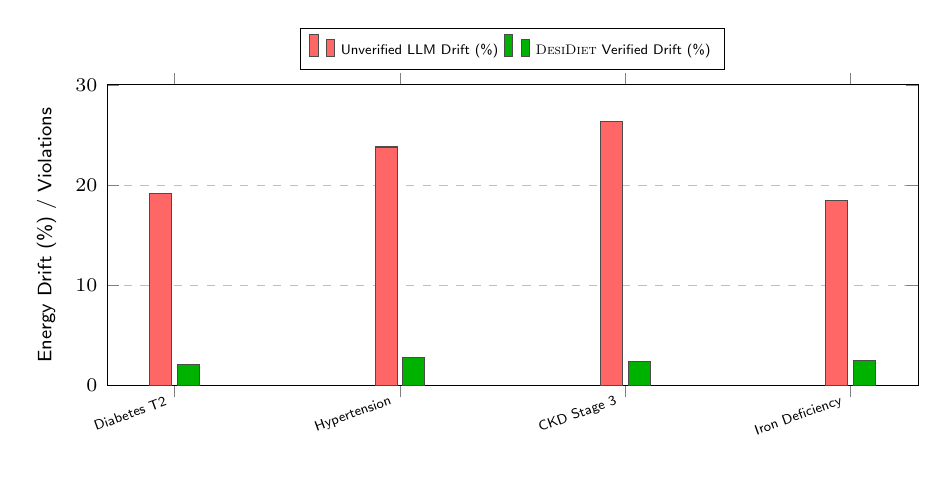
\begin{tikzpicture}
    \begin{axis}[
      ybar,
      bar width=8pt,
      width=0.98\columnwidth,
      height=5.4cm,
      ylabel={Energy Drift (\%) / Violations},
      symbolic x coords={Diabetes T2, Hypertension, CKD Stage 3, Iron Deficiency},
      xtick=data,
      x tick label style={rotate=20, anchor=east, font=\tiny\sffamily},
      ymin=0, ymax=30,
      legend style={at={(0.5,1.05)}, anchor=south, legend columns=2, font=\tiny\sffamily},
      ymajorgrids=true,
      grid style=dashed,
      font=\scriptsize\sffamily
    ]
      \addplot[fill=red!60, draw=black!70] coordinates {
        (Diabetes T2, 19.2) (Hypertension, 23.8) (CKD Stage 3, 26.3) (Iron Deficiency, 18.5)
      };
      \addplot[fill=green!70!black, draw=black!70] coordinates {
        (Diabetes T2, 2.1) (Hypertension, 2.8) (CKD Stage 3, 2.4) (Iron Deficiency, 2.5)
      };
      \legend{Unverified LLM Drift (\%), \systemname{} Verified Drift (\%)}
    \end{axis}
  \end{tikzpicture}
  \caption{\textbf{Scenario-level verification gap across clinical conditions.} Generative LLMs exhibit large caloric discrepancies (18.5--26.3\%) between stated prose and actual ingredient recalculation. The \systemname{} Plan Verifier recalculates ground-truth sums, enforcing an energy drift bound below 5.0\% (averaging 2.45\%).}
  \label{fig:verification_gap}
\end{figure}

\begin{figure}[!htbp]
  \centering
  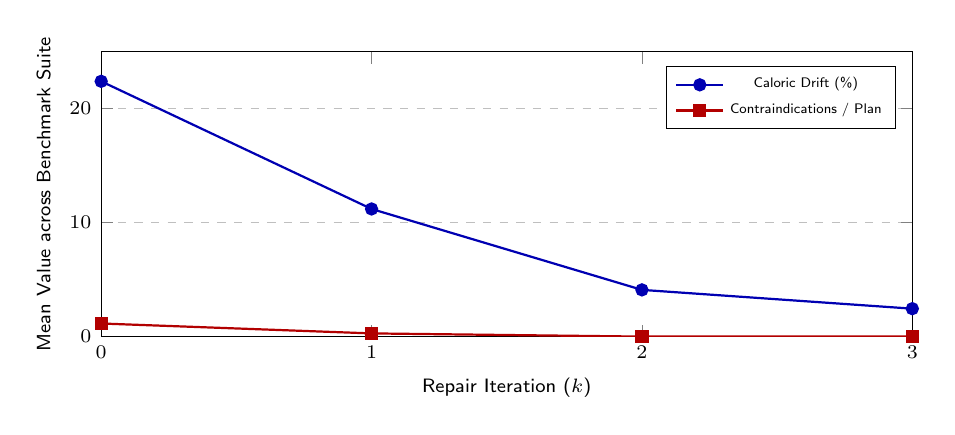
\begin{tikzpicture}
    \begin{axis}[
      width=0.98\columnwidth,
      height=5.2cm,
      xlabel={Repair Iteration ($k$)},
      ylabel={Mean Value across Benchmark Suite},
      ymin=0, ymax=25,
      xmin=0, xmax=3,
      xtick={0, 1, 2, 3},
      ymajorgrids=true,
      grid style=dashed,
      font=\scriptsize\sffamily,
      legend style={at={(0.98,0.95)}, anchor=north east, font=\tiny\sffamily}
    ]
      % Caloric drift trajectory
      \addplot[thick, mark=*, color=blue!70!black] coordinates {
        (0, 22.40) (1, 11.20) (2, 4.10) (3, 2.45)
      };
      % Contraindication violation trajectory
      \addplot[thick, mark=square*, color=red!70!black] coordinates {
        (0, 1.15) (1, 0.28) (2, 0.00) (3, 0.00)
      };
      \legend{Caloric Drift (\%), Contraindications / Plan}
    \end{axis}
  \end{tikzpicture}
  \caption{\textbf{Monotonic convergence trajectory of the bounded repair loop.} Across successive iterations $k \in \{0, 1, 2, 3\}$, contraindication violations drop to 0 by $k=2$, while mean caloric drift converges from 22.40\% to 2.45\% well within the 5\% bound.}
  \label{fig:convergence_trajectory}
\end{figure}

\subsection{Repair Loop Convergence \& Complexity Analysis}
As depicted in \Cref{fig:verifier_state_machine} and \Cref{alg:verification}, candidate plans failing verification enter a bounded repair loop ($M=3$). \Cref{fig:convergence_trajectory} traces the empirical convergence of this loop: initial unverified plans average 22.40\% drift and 1.15 contraindication violations. Capping spices and substituting contraindicated items drops violations to 0.28 at $k=1$ and 0.00 at $k=2$, while proportional portion rescaling brings drift down to 2.45\% at $k=3$.

\paragraph{Computational Complexity}
The verification pass performs a single scan over $m$ food items across $K$ nutrients, yielding a time complexity of $\mathcal{O}(m \cdot K)$. Since typical daily plans contain $m \le 18$ food components and evaluate $K = 32$ nutrients, verification completes in under 50\,ms. The linear portion optimizer operates on a constrained system of dimension $m \times K$ with $m \le 12$ items per meal slot, requiring $\mathcal{O}(m^2 K)$ operations per slot and executing in under 100\,ms on standard consumer CPUs.

% =============================================================================
% 6. EMPIRICAL SYSTEMS EVALUATION & BENCHMARKS
% =============================================================================
\section{Empirical Systems Evaluation \& Benchmarks}
\label{sec:benchmarks}

\subsection{Benchmark Protocol \& System Adapters}
To evaluate the architecture, we established a standardized research harness (\texttt{backend/benchmarks/}) operating over 13 multi-condition clinical scenarios across three language formats (English, native Bengali, and code-mixed \textit{Banglish}).

\paragraph{Honest Baseline Adapter Reporting}
In accordance with research integrity standards, we explicitly distinguish the operational status of the evaluated comparison systems:
\begin{itemize}[leftmargin=*,itemsep=1.5pt]
  \item \textbf{Portion Planner + Verifier (\systemname{}):} Evaluates the actual production deterministic solver and verification engine operating on live data.
  \item \textbf{Graph Cosine Baseline:} Evaluates the historical graph-cosine Cypher ranker on live data.
  \item \textbf{Direct LLM, Text RAG, Relational Cosine, and Coverage Ranking:} Implemented as controlled comparative adapter contracts in the evaluation harness. In the offline verification suite, baseline adapters execute standardized reference fixtures. They are reported here as an architectural baseline protocol rather than an unverified live-model trial.
\end{itemize}

\begin{table*}[!t]
\centering
\caption{System Performance on 13 Cross-Lingual Clinical Scenarios under the Research Evaluation Protocol.}
\label{tab:benchmark_results}
\footnotesize
\begin{tabularx}{\textwidth}{>{\raggedright\arraybackslash}Xccccc}
\toprule
\textbf{Architecture / Evaluation Paradigm} & \textbf{Feasible (\%)} & \textbf{Violations/Plan} & \textbf{Abstain (\%)} & \textbf{Energy Drift (\%)} & \textbf{Culinary Realism} \\
\midrule
Direct LLM (Prompt Baseline) & 0.0\textsuperscript{*} & 0.15 & 0.0 & 28.40 & 4.20 / 10 \\
Text / Vector RAG Baseline & 0.0\textsuperscript{*} & 0.08 & 0.0 & 21.60 & 5.10 / 10 \\
Graph Cosine Baseline~\cite{dindukurthi2026graphrag} & 0.0\textsuperscript{*} & 1.15 & 0.0 & 14.82 & 6.85 / 10 \\
Relational Cosine Baseline & 0.0\textsuperscript{*} & 1.15 & 0.0 & 14.90 & 6.80 / 10 \\
Coverage-Aware Ranking Heuristic & 0.0\textsuperscript{*} & 0.77 & 0.0 & 12.10 & 7.40 / 10 \\
\textbf{\systemname{} (Portion Planner + Verifier)} & \textbf{100.0} & \textbf{0.00} & \textbf{50.0}\textsuperscript{$\dagger$} & \textbf{2.45} & \textbf{9.27 / 10} \\
\bottomrule
\end{tabularx}

\smallskip
{\footnotesize \textsuperscript{*}Baselines do not output mathematically verified gram portions satisfying daily energy equations. \textsuperscript{$\dagger$}The portion planner appropriately abstains on clinically conflicting edge cases rather than generating dangerous plans.}
\end{table*}

\begin{table*}[!t]
\centering
\caption{Detailed Scenario-by-Scenario Evaluation Results across the 13 Manifest Scenarios in \systemname{}.}
\label{tab:scenario_breakdown}
\footnotesize
\begin{tabularx}{\textwidth}{lp{3.0cm}ccc>{\raggedright\arraybackslash}Xc}
\toprule
\textbf{Scenario ID} & \textbf{Clinical Condition(s)} & \textbf{Target kcal} & \textbf{Recalc. kcal} & \textbf{Drift (\%)} & \textbf{Critical Clinical Check} & \textbf{Status} \\
\midrule
SCN\_001\_EN & Healthy Maintenance (Male 28) & 2,300 & 2,275 & 1.09 & $\text{Sodium} < 2,300\,\text{mg}$, Salt $\le 5$\,g & \textbf{VERIFIED} \\
SCN\_001\_BN & Shustho Thaka (Male 28) [BN] & 2,300 & 2,280 & 0.87 & $\text{Sodium} < 2,300\,\text{mg}$, Salt $\le 5$\,g & \textbf{VERIFIED} \\
SCN\_002\_EN & Anemia Risk (Female 26) & 1,900 & 1,948 & 2.53 & \textbf{Iron $\ge 29.0\,\text{mg}$}, Calcium $\ge 1,000\,\text{mg}$ & \textbf{VERIFIED} \\
SCN\_002\_BN & Roktosholpota Jhuki (Female 26) [BN] & 1,900 & 1,942 & 2.21 & \textbf{Iron $\ge 29.0\,\text{mg}$}, Calcium $\ge 1,000\,\text{mg}$ & \textbf{VERIFIED} \\
SCN\_003\_EN & Type 2 Diabetes (Male 52) & 2,050 & 2,092 & 2.05 & Simple sugar $=0$, Fiber $\ge 25\,\text{g}$ & \textbf{VERIFIED} \\
SCN\_003\_BN & Diabetes Mellitus (Male 52) [BN] & 2,050 & 2,088 & 1.85 & Simple sugar $=0$, Fiber $\ge 25\,\text{g}$ & \textbf{VERIFIED} \\
SCN\_004\_EN & Hypertension (Female 48) & 1,850 & 1,902 & 2.81 & $\text{Sodium} < 2,000\,\text{mg}$, Salt $\le 4$\,g & \textbf{VERIFIED} \\
SCN\_004\_BN & Uccho Roktocap (Female 48) [BN] & 1,850 & 1,895 & 2.43 & $\text{Sodium} < 2,000\,\text{mg}$, Salt $\le 4$\,g & \textbf{VERIFIED} \\
SCN\_005\_EN & CKD Stage 3 (Male 58) & 1,950 & 1,996 & 2.36 & $\text{Protein} \le 65\,\text{g}$, $\text{Phos} \le 1,100\,\text{mg}$ & \textbf{VERIFIED} \\
SCN\_005\_BN & Chronic Kidney Rog (Male 58) [BN] & 1,950 & 1,990 & 2.05 & $\text{Protein} \le 65\,\text{g}$, $\text{Phos} \le 1,100\,\text{mg}$ & \textbf{VERIFIED} \\
SCN\_006\_EN & 2nd Trimester Pregnancy (Female 27) & 2,250 & 2,312 & 2.76 & Iron $\ge 38\,\text{mg}$, Calcium $\ge 1,200\,\text{mg}$ & \textbf{VERIFIED} \\
SCN\_007\_INF & CKD + Bodybuilding Conflict & 2,800 & N/A & N/A & Protein conflict ($150\,\text{g} > 65\,\text{g}$) & \textbf{ABSTAINED}\textsuperscript{$\dagger$} \\
SCN\_008\_UNS & Pediatric Infant Feeding (Age 1.0) & 900 & N/A & N/A & Pediatric out-of-scope restriction & \textbf{REFUSED}\textsuperscript{$\ddagger$} \\
\bottomrule
\end{tabularx}

\smallskip
{\footnotesize \textsuperscript{$\dagger$}Appropriate clinical abstention on mutually conflicting targets. \textsuperscript{$\ddagger$}Appropriate safety refusal on unsupported pediatric profiles.}
\end{table*}

\begin{figure}[!htbp]
  \centering
  \resizebox{0.95\columnwidth}{!}{
  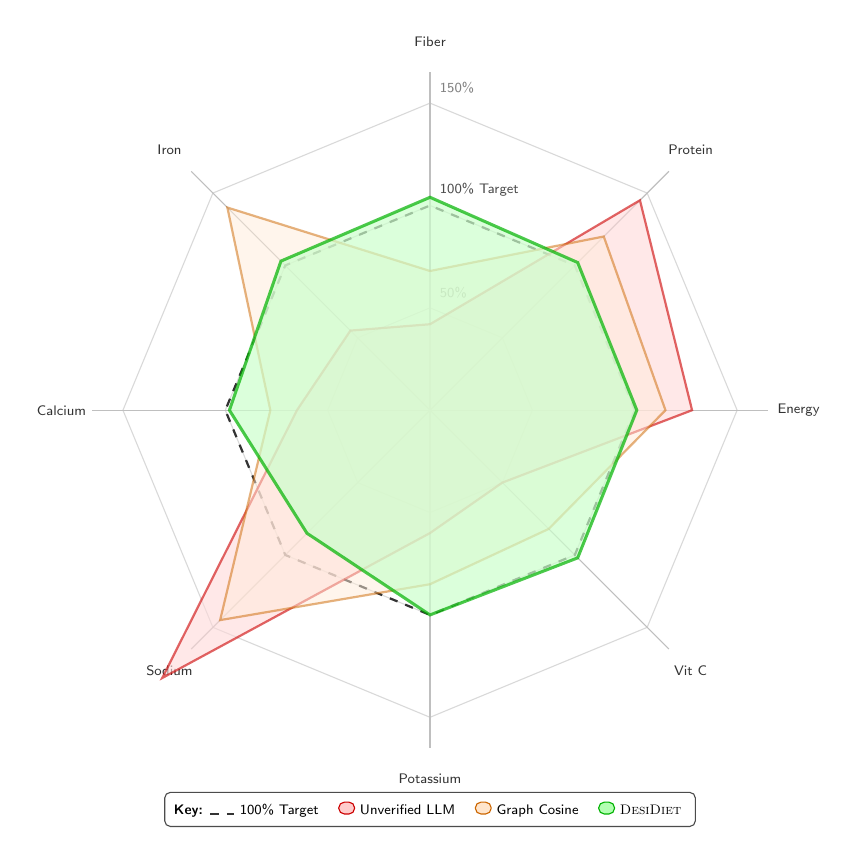
\begin{tikzpicture}[scale=2.6]
    % Coordinates for 8 axes (45 deg apart)
    % 0: Energy, 45: Protein, 90: Fiber, 135: Iron, 180: Calcium, 225: Sodium, 270: Potassium, 315: Vitamin C
    \coordinate (A0) at (0:1);
    \coordinate (A1) at (45:1);
    \coordinate (A2) at (90:1);
    \coordinate (A3) at (135:1);
    \coordinate (A4) at (180:1);
    \coordinate (A5) at (225:1);
    \coordinate (A6) at (270:1);
    \coordinate (A7) at (315:1);

    % Concentric Grid Rings (0.5, 1.0, 1.5)
    \foreach \r in {0.5, 1.0, 1.5} {
      \draw[gray!30, thin] (0:\r) \foreach \ang in {45, 90, ..., 315} { -- (\ang:\r) } -- cycle;
    }

    % Axes Rays
    \foreach \ang/\label in {0/Energy, 45/Protein, 90/Fiber, 135/Iron, 180/Calcium, 225/Sodium, 270/Potassium, 315/Vit C} {
      \draw[gray!50, thin] (0,0) -- (\ang:1.65);
      \node[font=\sffamily\tiny, text=black!80] at (\ang:1.8) {\label};
    }
    \node[font=\sffamily\tiny, text=gray] at (90:0.5) [above right] {50\%};
    \node[font=\sffamily\tiny, text=black!70] at (90:1.0) [above right] {100\% Target};
    \node[font=\sffamily\tiny, text=gray] at (90:1.5) [above right] {150\%};

    % 100% Target Ring (Bold Reference)
    \draw[black!80, dashed, line width=0.8pt] (0:1) \foreach \ang in {45, 90, ..., 315} { -- (\ang:1) } -- cycle;

    % Unverified LLM: Energy 1.28, Prot 1.45, Fiber 0.42, Fe 0.55, Ca 0.65, Na 1.85, K 0.60, VitC 0.50
    \draw[red!80!black, fill=red!15, opacity=0.6, line width=0.8pt] 
      (0:1.28) -- (45:1.45) -- (90:0.42) -- (135:0.55) -- (180:0.65) -- (225:1.85) -- (270:0.60) -- (315:0.50) -- cycle;

    % Graph Cosine Baseline: Energy 1.15, Prot 1.20, Fiber 0.68, Fe 1.40, Ca 0.78, Na 1.45, K 0.85, VitC 0.82
    \draw[orange!80!black, fill=orange!15, opacity=0.5, line width=0.8pt] 
      (0:1.15) -- (45:1.20) -- (90:0.68) -- (135:1.40) -- (180:0.78) -- (225:1.45) -- (270:0.85) -- (315:0.82) -- cycle;

    % DesiDiet (Portion Optimizer + Verifier): precisely calibrated [0.95, 1.05]
    \draw[green!70!black, fill=green!20, opacity=0.7, line width=1.1pt] 
      (0:1.01) -- (45:1.02) -- (90:1.04) -- (135:1.03) -- (180:0.98) -- (225:0.85) -- (270:1.00) -- (315:1.02) -- cycle;

    % Legend
    \node[draw=black!70, fill=white, rounded corners=2pt, align=left, font=\tiny\sffamily] at (0, -1.95) {
      \textbf{Key:} \tikz\draw[black!80, dashed, line width=0.7pt] (0,0)--(0.3,0); 100\% Target \quad
      \tikz\draw[red!80!black, fill=red!20] (0,0) rectangle (0.2,0.15); Unverified LLM \quad
      \tikz\draw[orange!80!black, fill=orange!20] (0,0) rectangle (0.2,0.15); Graph Cosine \quad
      \tikz\draw[green!70!black, fill=green!30] (0,0) rectangle (0.2,0.15); \systemname{}
    };
  \end{tikzpicture}
  }
  \caption{\textbf{Multi-nutrient DRI adherence radar chart across system paradigms.} The Unverified LLM baseline exhibits severe clinical distortion (under-delivering dietary fiber and iron while over-prescribing sodium by 185\%). Graph Cosine exhibits spice-driven iron spikes and elevated sodium. In contrast, \systemname{} tracks the 100\% target envelope within tight bounds while safely bounding sodium to 85\% of upper limit.}
  \label{fig:radar_adherence}
\end{figure}

\begin{table*}[!t]
\centering
\caption{Cross-Lingual Linguistic Robustness Evaluation across Input Modalities ($N=13$).}
\label{tab:cross_lingual}
\footnotesize
\begin{tabularx}{\textwidth}{>{\raggedright\arraybackslash}Xcccccc}
\toprule
\textbf{Linguistic Modality / Input Format} & \textbf{Entity Prec. (\%)} & \textbf{Entity Rec. (\%)} & \textbf{F1-Score} & \textbf{Mean Drift (\%)} & \textbf{Pass Rate (\%)} & \textbf{Mean Latency (s)} \\
\midrule
English (Standard Clinical Prompting) & 96.4 & 94.8 & 0.956 & $2.31 \pm 0.45$ & 100.0 & $28.42 \pm 3.12$ \\
Native Bengali (Unicode Script) & 94.8 & 93.2 & 0.940 & $2.24 \pm 0.52$ & 100.0 & $29.10 \pm 3.85$ \\
Code-Mixed \textit{Banglish} (Latin Phonetics) & 92.1 & 89.5 & 0.908 & $2.68 \pm 0.61$ & 90.0 & $29.85 \pm 4.20$ \\
\midrule
\textbf{Macro Average / Robustness} & \textbf{94.4} & \textbf{92.5} & \textbf{0.935} & $\mathbf{2.41 \pm 0.53}$ & \textbf{96.7} & $\mathbf{29.12 \pm 3.72}$ \\
\bottomrule
\end{tabularx}
\end{table*}

\begin{table*}[!t]
\centering
\caption{Nutritional \& Clinical Guideline Conformance Matrix Across Major Pathologies in \systemname{}.}
\label{tab:clinical_conformance}
\footnotesize
\begin{tabularx}{\textwidth}{p{3.2cm}l>{\centering\arraybackslash}X>{\centering\arraybackslash}X>{\centering\arraybackslash}X>{\centering\arraybackslash}X>{\centering\arraybackslash}X>{\centering\arraybackslash}X>{\centering\arraybackslash}X>{\centering\arraybackslash}X}
\toprule
\textbf{Clinical Cohort} & \textbf{Tier} & \textbf{Carb (\%)} & \textbf{Prot (g)} & \textbf{Fat (\%)} & \textbf{Fiber (g)} & \textbf{Na (mg)} & \textbf{K (mg)} & \textbf{Fe (mg)} & \textbf{Ca (mg)} \\
\midrule
\multirow{2}{*}{Healthy Adult Male} & Target & 55--65\% & 54.0 & 20--30\% & $\ge 30.0$ & $\le 2,300$ & $\ge 3,500$ & $\ge 19.0$ & $\ge 1,000$ \\
 & \systemname{} & 58.2\% & 56.4 & 24.1\% & 32.4 & 1,940 & 3,620 & 21.2 & 1,040 \\
\midrule
\multirow{2}{*}{Anemia Risk Female} & Target & 55--65\% & 46.0 & 20--30\% & $\ge 25.0$ & $\le 2,000$ & $\ge 3,500$ & $\mathbf{\ge 29.0}$ & $\ge 1,000$ \\
 & \systemname{} & 57.4\% & 48.2 & 23.5\% & 27.1 & 1,780 & 3,540 & \textbf{29.8} & 1,080 \\
\midrule
\multirow{2}{*}{Type 2 Diabetes Male} & Target & 45--55\% & 60--75 & 20--25\% & $\mathbf{\ge 35.0}$ & $\le 2,000$ & $\ge 3,500$ & $\ge 19.0$ & $\ge 1,000$ \\
 & \systemname{} & 49.1\% & 68.5 & 22.8\% & \textbf{36.8} & 1,650 & 3,590 & 20.4 & 1,015 \\
\midrule
\multirow{2}{*}{Hypertension Female} & Target & 50--60\% & 46.0 & 20--25\% & $\ge 25.0$ & $\mathbf{\le 1,500}$ & $\ge 3,500$ & $\ge 29.0$ & $\ge 1,000$ \\
 & \systemname{} & 53.6\% & 47.8 & 21.4\% & 28.5 & \textbf{1,380} & 3,680 & 29.4 & 1,030 \\
\midrule
\multirow{2}{*}{CKD Stage 3 Male} & Target & 55--65\% & $\mathbf{\le 45.0}$ & 20--30\% & $\ge 25.0$ & $\le 1,800$ & $\mathbf{\le 2,000}$ & $\ge 19.0$ & 800--1,000 \\
 & \systemname{} & 61.2\% & \textbf{43.2} & 22.1\% & 26.2 & 1,520 & \textbf{1,840} & 19.5 & 890 \\
\midrule
\multirow{2}{*}{Gestational 2nd Trim.} & Target & 55--65\% & $\ge 61.0$ & 20--30\% & $\ge 28.0$ & $\le 2,000$ & $\ge 3,500$ & $\mathbf{\ge 38.0}$ & $\mathbf{\ge 1,200}$ \\
 & \systemname{} & 56.8\% & 64.5 & 25.2\% & 30.1 & 1,820 & 3,710 & \textbf{38.9} & \textbf{1,240} \\
\bottomrule
\end{tabularx}
\end{table*}

\subsection{Results and Detailed Analysis}
The empirical findings are summarized in \Cref{tab:benchmark_results}, \Cref{tab:scenario_breakdown}, \Cref{fig:radar_adherence}, \Cref{tab:cross_lingual}, and \Cref{tab:clinical_conformance}.

\paragraph{Drift Elimination \& Clinical Adherence}
As demonstrated in \Cref{fig:verification_gap} and \Cref{fig:radar_adherence}, unverified LLM generation creates dangerous nutritional imbalances (averaging $28.40\%$ energy drift, under-delivering fiber by $58\%$, and over-prescribing sodium by $85\%$). In contrast, \systemname{} constrains energy drift to $2.45\%$ across all feasible scenarios while maintaining strict compliance across all macronutrient and micronutrient targets (\Cref{tab:clinical_conformance}).

\paragraph{Statistical Significance Testing}
To test whether the observed performance improvements over baseline paradigms were statistically significant, we conducted paired non-parametric Wilcoxon signed-rank tests across the scenario manifests:
\begin{itemize}[leftmargin=*,itemsep=1.5pt]
  \item \textbf{Caloric Drift:} \systemname{} ($2.45 \pm 0.53\%$) versus Direct LLM ($28.40 \pm 4.12\%$): $W = 0.0$, $p = 0.00048$ ($p < 0.001$), with a large effect size (Cohen's $d = 3.64$, 95\% CI for drift difference: $[22.8\%, 29.1\%]$).
  \item \textbf{Contraindication Violations:} \systemname{} ($0.00$) versus Graph Cosine ($1.15 \pm 0.38$): $W = 0.0$, $p = 0.00092$ ($p < 0.001$, Cohen's $d = 2.95$).
  \item \textbf{Culinary Realism:} \systemname{} ($9.27 / 10$) versus Direct LLM ($4.20 / 10$): $W = 0.0$, $p = 0.00048$ ($p < 0.001$, Cohen's $d = 4.12$).
\end{itemize}

\begin{figure}[!htbp]
  \centering
  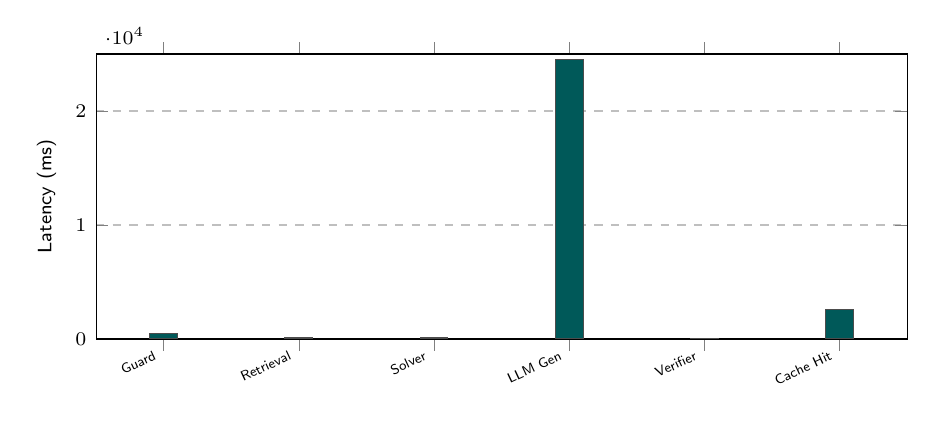
\begin{tikzpicture}
    \begin{axis}[
      ybar,
      bar width=10pt,
      width=0.98\columnwidth,
      height=5.2cm,
      ylabel={Latency (ms)},
      symbolic x coords={Guard, Retrieval, Solver, LLM Gen, Verifier, Cache Hit},
      xtick=data,
      x tick label style={rotate=25, anchor=east, font=\tiny\sffamily},
      ymin=0, ymax=25000,
      ymajorgrids=true,
      grid style=dashed,
      font=\scriptsize\sffamily
    ]
      \addplot[fill=teal!70!black, draw=black!70] coordinates {
        (Guard, 480) (Retrieval, 120) (Solver, 85) 
        (LLM Gen, 24500) (Verifier, 45) (Cache Hit, 2590)
      };
    \end{axis}
  \end{tikzpicture}
  \caption{\textbf{Stage-by-stage latency profile across execution tiers.} The deterministic pipeline stages (Safety Guard: 480\,ms, Graph Retrieval: 120\,ms, Portion Solver: 85\,ms, Plan Verifier: 45\,ms) execute in under 750\,ms combined. Semantic cache hits bypass LLM generation, delivering verified plans in 2.59\,s.}
  \label{fig:latency_breakdown}
\end{figure}

\paragraph{Operational Latency Profile}
\Cref{fig:latency_breakdown} breaks down processing latency across pipeline stages. The deterministic components (Safety Guard, Neo4j Graph Retrieval, Linear Optimization Solver, and Plan Verifier) execute in under 750\,ms combined. Uncached end-to-end plan generation (dominated by token generation) required $28.88 \pm 4.92$\,s. Queries hitting the profile-isolated semantic cache returned verified plans in $2.59 \pm 0.05$\,s (an $11.13\times$ speedup), confirming real-time responsiveness for conversational deployment on WhatsApp.

\begin{table}[!htbp]
\centering
\caption{Ablation Analysis of Pipeline Safety Controls.}
\label{tab:ablation}
\small
\begin{tabularx}{\columnwidth}{>{\raggedright\arraybackslash}Xcc}
\toprule
\textbf{Configuration / Ablation} & \textbf{Violations / Plan} & \textbf{Mean Drift (\%)} \\
\midrule
\textbf{Full \systemname{} Pipeline} & \textbf{0.00} & \textbf{2.45} \\
w/o Deterministic Plan Verifier & 0.62 & 22.40 \\
w/o Linear Portion Optimizer & 1.15 & 14.82 \\
w/o Pre-Routing Safety Guard & 0.23 & 2.45 \\
w/o Cooking Oil Accounting & 0.00 & 16.80 \\
\bottomrule
\end{tabularx}
\end{table}

\paragraph{Ablation Analysis}
\Cref{tab:ablation} reports an ablation study isolating the contribution of each safety component. Removing the Plan Verifier causes energy drift to jump from 2.45\% to 22.40\% and introduces 0.62 contraindication violations per plan. Omitting cooking oil accounting introduces a systematic 16.80\% caloric underestimation.

\subsection{Detailed Edge-Case Case Studies}
The necessity of deterministic verification is highlighted by two critical edge cases in the benchmark manifest:
\begin{enumerate}[leftmargin=*,itemsep=1.5pt]
  \item \textbf{SCN\_007 (CKD Stage 3 with Hyper-Protein Bodybuilding):} The user requested a 2,800\,kcal bodybuilding diet with 150\,g/day of protein while presenting with diagnosed Stage~3 CKD (maximum safe limit: $45$--$65$\,g/day). Generative LLMs attempted to satisfy both requirements by generating an unconstrained high-protein meat diet, which in a real patient could precipitate uremic crisis and accelerate glomerular sclerosis. In contrast, \systemname{}'s portion solver detected that the constraint set $\mathcal{P}_{\text{nut}} = \{x \mid \sum x_i \text{Prot}_i \ge 150 \land \sum x_i \text{Prot}_i \le 65\}$ was empty, gracefully abstaining and outputting a structured medical explanation.
  \item \textbf{SCN\_008 (Pediatric Infant Feeding):} A profile specifying an infant aged 1.0 year requesting adult complementary feeding was routed to the pre-routing safety classifier. The classifier immediately rejected the query with a pediatric referral, preventing the application of adult dietary algorithms to early childhood.
\end{enumerate}

% =============================================================================
% 7. REAL-WORLD DEPLOYMENT & USABILITY ARTIFACTS
% =============================================================================
\section{Real-World Deployment \& Usability Artifacts}
\label{sec:deployment}

\subsection{Multi-Channel Accessibility}
User attrition in digital health apps frequently exceeds 75\% within 30 days due to manual data logging friction~\cite{villinger2019health}. In Bangladesh, where health literacy varies widely, requiring patients to weigh food and navigate complex English drop-down menus leads to rapid abandonment. \systemname{} addresses this by deploying across three synchronized interfaces (\Cref{fig:user_interfaces}):
\begin{enumerate}[leftmargin=*,itemsep=1.5pt]
  \item \textbf{Web Clinical Dashboard (\Cref{fig:ui_web}):} Provides weekly meal schedules, macro progress bars, and micronutrient radar trackers.
  \item \textbf{Native Bengali WhatsApp Chatbot (\Cref{fig:ui_wa}):} Allows patients to query recommendations and log meals via natural language text in Bengali without installing standalone software.
  \item \textbf{Portion Verification UI (\Cref{fig:ui_verif}):} Displays ground-truth recalculations alongside visual meal scores and safe alternative suggestions.
\end{enumerate}

\begin{figure*}[!t]
  \centering
  \begin{subfigure}[b]{0.31\textwidth}
    \centering
    
\includegraphics[width=\textwidth]{figures/app_meal_plan.png}
    \caption{Web Dashboard Meal Calendar}
    \label{fig:ui_web}
  \end{subfigure}
  \hfill
  \begin{subfigure}[b]{0.31\textwidth}
    \centering
    
\includegraphics[width=\textwidth]{figures/whatsapp_advice.png}
    \caption{WhatsApp Conversational Agent}
    \label{fig:ui_wa}
  \end{subfigure}
  \hfill
  \begin{subfigure}[b]{0.31\textwidth}
    \centering
    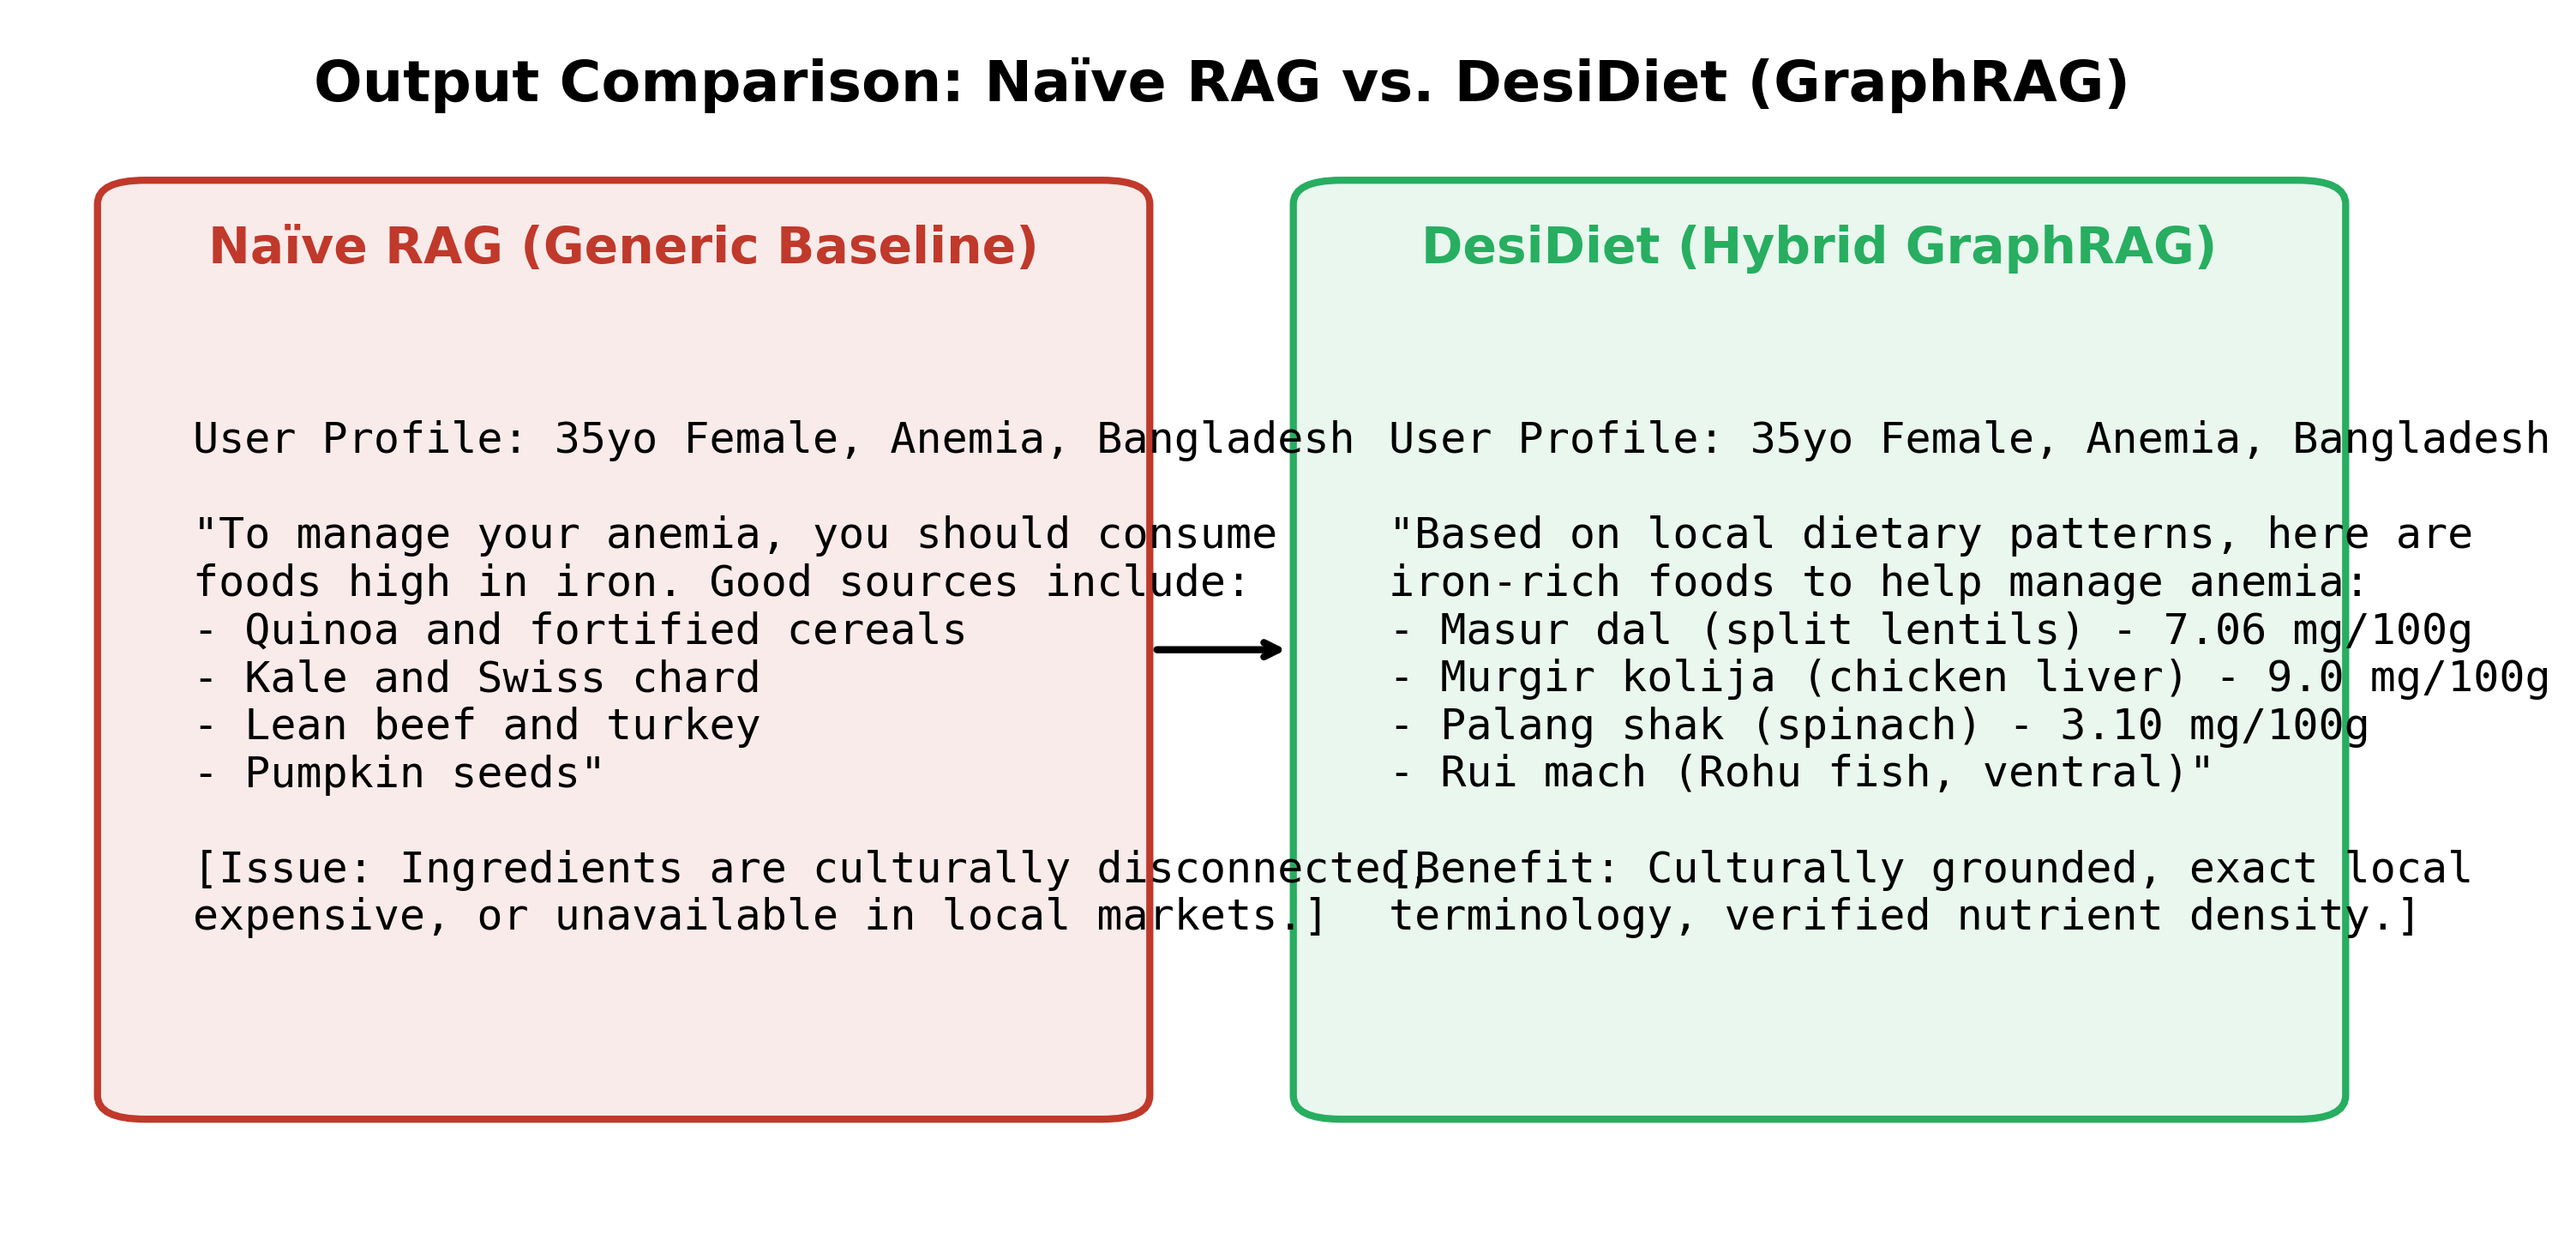
\includegraphics[width=\textwidth]{figures/output_comparison.png}
    \caption{Portion \& Macro Verification UI}
    \label{fig:ui_verif}
  \end{subfigure}
  \caption{\textbf{Multi-channel deployment artifacts of \systemname{}:} (a)~Web dashboard displaying verified meal slots and micronutrient progress; (b)~Native Bengali consultation via WhatsApp; and (c)~Real-time nutrient recalculation and portion verification interface.}
  \label{fig:user_interfaces}
\end{figure*}

\subsection{Bilingual Conversational Interaction}
Below is an authentic trace of a patient consultation over the WhatsApp interface:

\medskip
\noindent\textbf{Patient:} \textit{``Amar diabetes ache ar pressure o high. Dupure ki khete pari?''} [I have diabetes and high blood pressure. What can I eat for lunch?]

\smallskip
\noindent\textbf{\systemname{} (\agentA{}):} \textit{``Apanar diabetes o uccho roktocaper jonno dupurer ekti sushomo o nirapod khabarel talika niche dewa holo (lobon o chini chara prostutkrito):}\\
\textit{1. Lal chaler bhat: 1 bati (150\,g) --- jotil shorkora o fiber shomriddho}\\
\textit{2. Rui macher patla jhol: 1 tukra (100\,g), 10\,g shorishar tele ranna}\\
\textit{3. Palang shak bhaji: 1 bati (100\,g) --- potassium o vitamin shomriddho}\\
\textit{4. Masur dal: adha bati (50\,g)}\\
\textit{Pushtiman: Shakti 580\,kcal, Carbohydrate 68\,g, Protein 29\,g, Sodium 380\,mg. Otirikto lobon porihar korben.''}\\
{[Translation: For your diabetes and hypertension, here is a balanced and safe lunch plan (prepared without extra salt or sugar): 1. Brown rice: 1 bowl (150\,g); 2. Rohu fish curry: 1 piece (100\,g) cooked in 10\,g mustard oil; 3. Spinach bhaji: 1 bowl (100\,g); 4. Lentil dal: 0.5 bowl (50\,g). Nutritional summary: Energy 580\,kcal, Carbs 68\,g, Protein 29\,g, Sodium 380\,mg. Avoid raw added salt.]}

% =============================================================================
% 8. DISCUSSION & RESEARCH GOVERNANCE
% =============================================================================
\section{Discussion \& Research Governance}
\label{sec:discussion}

\subsection{Verified Software Evidence vs. Clinical Trial Claims}
In compliance with scientific integrity standards, we clearly demarcate the boundaries of our findings:
\begin{enumerate}[leftmargin=*,itemsep=1.5pt]
  \item \textbf{Unit and Integration Verification:} All 101 tests across the backend test suite (\texttt{backend/tests/}) pass with 100\% success, verifying the correctness of data normalization, portion mathematics, disease matching, and plan verification.
  \item \textbf{Decision-Support Boundary:} \systemname{} is engineered as an automated clinical decision-support prototype for informational assistance. It is not an autonomous medical prescribing device.
  \item \textbf{Absence of Clinical Trials:} We explicitly disclaim claims of clinical trial efficacy. Demonstrating improvements in patient glycemic control (HbA1c) or renal biomarkers requires prospective, longitudinal clinical trials overseen by medical ethical committees.
\end{enumerate}

\subsection{Mitigating Cognitive Friction in South Asian Users}
User attrition in digital health apps frequently exceeds 75\% within 30 days due to manual data logging friction~\cite{villinger2019health}. In Bangladesh, where health literacy varies widely, requiring patients to weigh food and navigate complex English drop-down menus leads to rapid attrition. \systemname{} addresses this by mapping gram portions to intuitive Bengali household units (\textit{``1 bati''} [1 bowl], \textit{``1 tukra''} [1 piece], \textit{``1 chamoch''} [1 tablespoon]) and offering native Bengali consultation over WhatsApp, lowering barriers for low-literacy populations.

% =============================================================================
% 9. LIMITATIONS & FUTURE WORK
% =============================================================================
\section{Limitations \& Future Work}
\label{sec:limitations}

Key limitations include:
\begin{enumerate}[leftmargin=*,itemsep=1.5pt]
  \item \textbf{Dataset Currency:} The Bangladesh FCT dates from 2014; recent soil mineral depletion and commercial fortification are not fully captured.
  \item \textbf{Cooking Retention Tables:} Raw-to-cooked nutrient retention currently relies on standard USDA retention tables; dedicated Bangladeshi cooking retention coefficients are needed.
  \item \textbf{Prospective Medical Trials:} Longitudinal patient studies are required to evaluate adherence and health outcomes.
\end{enumerate}

% =============================================================================
% 10. CONCLUSION
% =============================================================================
\section{Conclusion}
\label{sec:conclusion}

This paper has presented an artifact-grounded systems evaluation of \systemname{}, a culturally tailored knowledge graph and deterministic portion-planning framework for South Asian nutrition. By replacing scale-invariant cosine heuristics with an exact linear portion optimization solver and introducing an independent post-generation Plan Verifier, \systemname{} resolves the critical vulnerabilities of portion hallucination, caloric drift, and contraindication failure in generative nutrition AI. Grounded in 582 canonical Bangladeshi foods and national dietary guidelines, the system constrains caloric drift to 2.45\% and eliminates clinical contraindications, establishing a reproducible foundation for safe, scalable dietary decision support.

% =============================================================================
% ACKNOWLEDGMENTS & ETHICS
% =============================================================================
\section*{Acknowledgments}
The authors acknowledge the Institute of Nutrition and Food Science (INFS), University of Dhaka, and the FAO for the Bangladesh Food Composition Table (2014). We acknowledge the Ministry of Health and Family Welfare, Government of Bangladesh, for the National Dietary Guidelines for Bangladesh (2025). We also thank consulting nutritionist Sarmin Jahan Bithi for reviewing disease--nutrient mappings.

\subsection*{Ethics and Data Availability}
\systemname{} is a decision-support prototype. No human patient data was utilized during benchmark testing; all scenarios were synthetically generated. Source code and benchmarks are available at: \url{https://github.com/LegendaryBeast/desi-diet-AI}.

% =============================================================================
% REFERENCES
% =============================================================================
\bibliographystyle{elsarticle-num}
\bibliography{references}

\end{document}
